\documentclass[10pt, twoside, openright]{memoir}
%\documentclass[9pt, twoside, openright, showtrims]{memoir}

\setstocksize{11in}{8in}
\settrimmedsize{9in}{8in}{*}
\settrims{0.7in}{0in}
\settypeblocksize{7.5in}{6.3in}{*}
\setlrmargins{.85in}{*}{*}
\setulmargins{*}{.6in}{*}
\setheadfoot{\onelineskip}{2\onelineskip}
\setheaderspaces{*}{2\onelineskip}{*}

\checkandfixthelayout

\makeatletter
\DeclareOldFontCommand{\rm}{\normalfont\rmfamily}{\mathrm}
\DeclareOldFontCommand{\sf}{\normalfont\sffamily}{\mathsf}
\DeclareOldFontCommand{\tt}{\normalfont\ttfamily}{\mathtt}
\DeclareOldFontCommand{\tt}{\smallfont\ttfamily}{\texxttt}
\DeclareOldFontCommand{\bf}{\normalfont\bfseries}{\mathbf}
\DeclareOldFontCommand{\it}{\normalfont\itshape}{\mathit}
\DeclareOldFontCommand{\sl}{\normalfont\slshape}{\@nomath\sl}
\DeclareOldFontCommand{\sc}{\normalfont\scshape}{\@nomath\sc}
\makeatother

% \usepackage{xcolor, calc, graphicx, soul, fourier, verbments, makeidx, mflogo}
\usepackage{xcolor, calc, graphicx, soul, minted, makeidx, mflogo, 
  pstricks, minitoc, amsmath, amssymb, pst-poly, longtable, tikz, titlesec,
scalerel, stackengine, microtype}
\usetikzlibrary{shapes, arrows, calc}
% Define block styles
\tikzstyle{decision} = [diamond, draw,
  text width=4.5em, text badly centered, node distance=3cm, inner sep=0pt]
\tikzstyle{startstop} = [rectangle, draw, 
  text width=5em, text centered, rounded corners, minimum height=2em]
\tikzstyle{line} = [draw, -latex']
\tikzstyle{cloud} = [draw, ellipse, node distance=3cm,
  minimum height=0.5cm]
\tikzstyle{io} = [trapezium, trapezium left angle=70, trapezium right
  angle=110, minimum width=0.5cm, minimum height=0.5cm, text centered, draw=black,
]
\tikzstyle{process} = [rectangle, minimum width=1cm, minimum height=0.5cm, text
  centered, draw=black]
\tikzstyle{arrow} = [->,>=stealth]

\newcommand\dangersign[1][2ex]{%
  \renewcommand\stacktype{L}%
  \scaleto{\stackon[1.3pt]{\color{red}$\triangle$}{\tiny !}}{#1}%
}

\let\footruleskip\undefined
\usepackage{fancyhdr}
\usepackage{fancyvrb}
\pagestyle{fancy}
\usepackage[shellescape, latex]{gmp}
\showtrimson

\definecolor{niceblack}{rgb}{.1, .1, .1}
\definecolor{webred}{rgb}{.7,0,0}
\definecolor{webbg}{rgb}{1,.8,.2}
\definecolor{bootstrapurl}{rgb}{0,.5,.75}
\definecolor{nicered}{rgb}{.7,0,0}
\definecolor{nicegreen}{rgb}{.129,.447,.149}
\definecolor{niceblue}{rgb}{0, 0, .6}
\definecolor{niceyellow}{rgb}{1,1,.95}
\color{niceblack}
\usepackage[colorlinks]{hyperref}
\hypersetup{%
  pdftitle={C Programming with C11},
  pdfauthor={Shiv S. Dayal},
  pdfkeywords={C, Programming},
  bookmarksnumbered,
  pdfstartview={FitH},
  urlcolor=cyan,
  linkcolor=cyan,
}%
\setlength{\tabcolsep}{10pt}
\renewcommand{\arraystretch}{1.5}

\renewcommand{\chaptermark}[1]{%
  \markboth{#1}{}}
\renewcommand{\sectionmark}[1]{%
  \markright{#1}{}}

\makeatletter
\newlength\dlf@normtxtw
\setlength\dlf@normtxtw{\textwidth}
\def\myhelvetfont{\def\sfdefault{mdput}}
\newsavebox{\feline@chapter}
\newcommand\feline@chapter@marker[1][4cm]{%
  \sbox\feline@chapter{%
    \resizebox{!}{#1}{\fboxsep=1pt%
      \colorbox{cyan}{\color{white}\bfseries\sffamily\thechapter}%
  }}%
  \rotatebox{90}{%
    \resizebox{%
      \heightof{\usebox{\feline@chapter}}+\depthof{\usebox{\feline@chapter}}}%
              {!}{\scshape\so\@chapapp}}\quad%
  \raisebox{\depthof{\usebox{\feline@chapter}}}{\usebox{\feline@chapter}}%
}
\newcommand\feline@chm[1][4cm]{%
  \sbox\feline@chapter{\feline@chapter@marker[#1]}%
  \makebox[0pt][l]{% aka \rlap
    \makebox[1cm][r]{\usebox\feline@chapter}%
}}
\makechapterstyle{daleif1}{
  \renewcommand\chapnamefont{\normalfont\HUGE\sffamily\scshape\raggedleft\so}
  \renewcommand\chaptitlefont{\normalfont\HUGE\sffamily\bfseries\scshape\color{cyan}}
  \renewcommand\chapternamenum{}
  \renewcommand\printchaptername{}
  \renewcommand\printchapternum{\null\hspace*{5.5in}\feline@chm[1cm]\par}
  \renewcommand\afterchapternum{\par\vskip\midchapskip}
  \renewcommand\printchaptertitle[1]{\chaptitlefont\raggedleft ##1\par}
}
\makeatother
\chapterstyle{daleif1}

\title{\sffamily\color{cyan}\HUGE{\textbf{Computer Programming with 
      GNU/Linux}}\\\vspace*{1cm}\Large{Vol. I}\\\vspace*{1cm}\LARGE{\textbf{Informal
      C Programming}}\vspace*{2cm}}
\author{\vspace*{1cm}\LARGE{Shiv S. Dayal}}
\date{}
\titleformat{\section}
  {\normalfont\sffamily\Large\bfseries\color{cyan}}
  {\thesection}{0em}{}
\titleformat{\subsection}
  {\normalfont\sffamily\large\bfseries\color{cyan}}
  {\thesection}{0em}{}
\titleformat{\subsubsection}
  {\normalfont\sffamily\large\bfseries\color{cyan}}
  {\thesection}{0em}{}
\titleformat{\subsubsubsection}
  {\normalfont\sffamily\bfseries\color{cyan}}
  {\thesection}{0em}{}
%\renewcommand{\ttdefault}{pcr}
\setlength{\parskip}{1em}
%\renewcommand{\rmdefault}{ptm}
%\renewcommand{\rmdefault}{phv}
\usepackage{fontspec}
%\setmainfont[Ligatures=TeX,Scale=1.1]{Times}
\setmonofont[Ligatures=TeX,Scale=.90]{Courier}
\setsansfont{Helvetica}
\renewcommand{\contentsname}{Table of Contents}
\makeindex
\setcounter{secnumdepth}{5}
\usepackage{etoolbox}
\makeatletter
\preto{\@verbatim}{\topsep=0pt \partopsep=0pt }
\makeatother
\begin{document}
\minitoc
\minilof
\minilot
\maketitle
\thispagestyle{empty}
\pagestyle{empty}
\vfill
\newpage
\vspace*{6in}
Copyright, \copyright~ Shiv Shankar Dayal, 2011. All rights reserved.\\\\
Permission is granted to copy, distribute and/or modify this document under the
terms of the GNU Free Documentation License, Version 1.3 or any later version
published by the Free Software Foundation; with no Invariant Sections, no
Front-Cover Texts, and no Back-Cover Texts. A copy of the license is included
in the section entitled ``GNU Free Documentation License''.
\newpage
\vspace*{2in}
\begin{center}
  \Large \it Dedicated to my family\\and Free Software Community
\end{center}
\newpage
\setcounter{page}{1}
\pagenumbering{roman}
\tableofcontents
\newpage
\listoffigures
\newpage
\listoftables
% \newpage
% \listofpyglistings
\newpage
\pagestyle{fancy}
\frontmatter
\setcounter{page}{1} 
\pagenumbering{roman}
%\chapter{Preface}
I welcome you to this pdf version of 
\url{https://10hash.com/books/c/} which is a complete rewrite. That 
was my first attempt to write at such a large scale and therefore there were 
many deficiencies in that version which I hope have been countered and
corrected in this version. In the HTML version I had put a lot of emphasis on 
specification. However, the feedback which I got from some of my readers is 
that it has become complicated and is not suitable for beginners. After 
thinking over it I found that it is the order of chpaters which needs to be 
corrected and a lot more examples and exercises need to be there.

In this rewrite I will arrange the chapters in a different way. The empahsis on 
specification will be treated in the last part of book.

\section*{What this book contains?}
This book is about C programming language. In this book I have explained the
syntax of C programming language. But it is not only for learning about
language but how to learn to program using C programming language is also
there. In this book we will follow latest ISO specification of C which is
popularly known as C11.

\section*{Who should read this book?}
People interested in learning C should read this. Anybody can read this book
who has little background on Mathematics. I would say high school education is
sufficient for reading it. So this book is for both beginners and experts
alike. For experts advanced concepts have been presented and also a reference
to standard library has been given along with its usage.

\section*{How to read this book?}
Well, learning programming is like learning a new language and then solving
problems is like Mathematics. So the latter is more important as unless you can
solve the problem on pen and paper, you cannot solve the problems using
C. However, the focus of this book is to explain the features and syntax of C
programming language not on how to solve the problem. To get a good grasp
on the contents of the book one should read the theory first then look at the
examples given and try to understand and run them and in the end attempt
the problems. If you cannot solve the problems then lookup the solution and
try to understand. In case of any problem please log on to my personal
question/answer website \url{http://kunjika.libreprogramming.org/} to get
more help.

\section*{Acknowledgements}
I am in great debt of my family and free software community because both of
these groups have been integral part of my life. Family has prvided direct
support while free software community has provided the freedom and freed me
from the slavery which comes as a package with commercial software. I am
especially grateful to my wife, son and parents because it is their time which
I have borrowed to put in the book. To pay my thanks from free software
community  I will take one name and that is Richard Stallman who started all
this  and is still fighting this never-ending war. When I was doing the Algebra
book then I realized how difficult it is to put Math on web in HTML format and
why Donald Knuth wrote \TeX{}. Also, \TeX{} was one of the first softwares to
be released as a free software. HTML has not yet matured to represent
mathematical content. MathML is supported by Mozilla. Webskit browsers started
supporting  then dropped and I would refrain to comment on commercial browser's support which do not even comply to starndard because they think they are the standards tehmselves and others will bend to their will.

Now as this book is being written using \LaTeX{}~ so obviously Leslie Lamport
and all the people involved with it have my thanks along with Donald Knuth. I
use Emacs with Auctex and hope that someday I will use it in a much more
productive way someday.

I have used TikZ as a tool for drawing all the diagrams. It is a wonderful
package and works very nicely. I have great appreciation for its author Till
Tantau.

%For syntax highlighting I have used \texttt{Verbatim} \LaTeX{} package which
%uses \texttt{pygments} as its backend. You can modify it and make it look
%different both at \LaTeX{} and \texttt{pygments} level. Thanks to the
%respective package authors.

For errors and suggestion please email me at
\href{mailto:shivshankar.dayal@gmail.com}{shivshankar.dayal@gmail.com} where I
will try to respond to each mail as
much as possible. Please use your real names in email not something like
coolguy. As an alternative you can report it at
\url{https://10hash.com} where a question/answer website is maintained.
\begin{flushright}
Shiv Shankar Dayal\\
Nalanda,\\
India, 2015
\end{flushright}

\newpage
\mainmatter
\pagenumbering{arabic}
%\chapter{Introduction}
C programming language is a relatively low-level programming language with an
inclination towards system programming. This book will try to serve both as a
tutorial and reference of C programming language. If you have not programmed
earlier then you should read in linear manner. Even if you have programmed it
would be better if you read the book in linear fashion because there are
certain points which you may miss if you skip chapters. Of all popular
mainstream languages C, and Lisp are two oldest but we cannot really say that
Lisp is really popular. It has a niche area(artificial intelligence) and it is
there for that. So let me redefine my statement. Of all general-purpose and
popular programming language C is the oldest. FORTRAN is another very old
language but it is not general purpose programming language. So what makes C so
special that it is still out there. Well, C and Unix were born almost together
in early 1970s. Then Unix was ported in C and the notion that operating systems
can be only written in assembly language, because it has to do time critical
things, was destroyed. After that Unix became very popular. Then when C++ was
not yet there Windows was written in C and more and more programs were written
in C. It might have been the case that Microsoft and Apple would have written
their OS in C++ had it been there. So, essentially what happened that there is
a lot of code base which is there in C. Also, C++'s backward compatibility is
one of the reasons why C++ is so popular. When C was invented there was no
structured programming language and code was mostly written in assembly. With C
it gave the power of assembly and benefits of structured language like code
reuse, modularity, and portability among others. Because of these reasons C
became immensely popular and is still popular. 

C is simple, small, succinct. It may be dirty but is quick. It may have its
quirks but it is a success. C is really so simple yet so deceptive. It will
take one years of programming to really thoroughly understand it.

C is currently described by ISO\/IEC 9899:2011 which you can buy on web or you
can get the draft revision
\url{http://www.open-std.org/jtc1/sc22/wg14/www/docs/n1570.pdf}. It
is not necessary to buy the specification as draft is very much similar. I will
refer to specification in the form of (§ iso.x.x.x.x) to point to sections
where exact information is discussed. Note that specification is written for
accuracy and the language is not trivial to understand. At the same time, it
does not directly address programmers but compiler writers because there are
certain decisions which specification does not make but rather leaves for
compiler authors' decision.

\section{Why C?}
Because it is the most common denominator. Any language be it C++, Java, Perl,
Python etc have got bindings in C. Whenever you are willing to extend these
languages you need to know C. Also, if by any chance you are going towards
system programming you need to C. C is everywhere. There is no escape from
learning it; it does not matter whether you like it or not. 

There is one more important point worth noting here is that C++ is far more
complex compared to C. It is generally accepted that one should not try to
learn C++ as one's first programming language. If you search web then you will
find that many great computer scientists like Ken Thompson, Richard Stallman,
Donald Knuth etc. clearly say that they do not like C++ because it is overly
complex. Also, the runtime(virtual functions) calculations of C++ make it
slightly slower than C. However, C++ has its own strengths and it excels as
well if used properly. Wherever there is a memory constraint or extreme high
performance is needed C is preferred. The simple syntax of C means its code is
very verbose for programmer in the sense that if you read code then you can
very easily see what instructions the code is going to translate into. 

It is very easy to write interfaces to other languages because other languages
expose there objects in terms of C structures not the other way around. The
reason for this is huge popularity of C, maturity and large code base. 

One more important feature is portability. Note that if you want your program
to have high degree of portability then you should not use C99 features but
rather ANSI C because ANSI C compilers are available on most platforms. Even
though Java claims to be portable or other interpreted languages they are
limited by the fact that the interpreters or VMs(JVM in case of Java) is not
available on all the platforms. Therefore, C is the MOST portable language.

One of the advantages with C is that since it is very old a lot of software has
been written using it. GNU/Linux for example uses C for its kernel. GNOME which
is one of the desktop environments of GNU/Linux is also written in C. The fact
is that since a lot of libraries are available in C thus it makes a lot of work
very easy to do in C since the infrastructure or ecosystem is developed and
mature. At the same time, since C is taught in many colleges and universities
as first course in programming a lot of people know C thus if you are writing
free(as in freedom) software then you have a much higher chance of getting
support if you write your code in C.

\section{History}
C was formally delivered to this world in 1972 and conceived by Dennis
MacAlistair Ritchie in 1968. What happened was there was a project for
development of a text processor and GE-645 was bought by AT\&T Bell Labs. At
that time Ken Thompson had developed a game called ``Space Travel''. Then they
had another machine PDP-11. Before that they had PDP-7. Now all the time the
code for ``Space Travel'' had to be rewritten and also the Unix had to be
ported. So when C was invented it was used to write Unix code in C. And then
``Space Travel''. I do not know what was the real motivation the language, the
OS or the game. But such is the story. Also, I have not studied much in this 
about the exact events. In 1972 C was formally announced. C takes its features
from BCPL a language by Martin Richard and B by Ken Thompson. AT\&T Bells labs
gave Unix and a C compiler to many universities at a normal fees and it grew
with leaps and bounds from there and became a ubiquitous language. For many
years ``The C Programming Language'' served as a reference of C. Later it was
standardized by ANSI and then by ISO standards. A very detailed history of C
programming language can be found at
\url{http://cm.bell-labs.com/cm/cs/who/dmr/chist.html} which has been described
by Dennis Ritchie himself.
\index{Dennis Ritchie}
\index{Ken Thompson}

\section{Comparison with Other Languages}
C is a structured, statically typed, somewhat low-level, high-performance
compiled language. It does not support object-oriented programming like most
modern programming including C++, Java, Perl, Python, Ruby etc. However, that
does not mean you cannot do object-oriented programming in C. It is just that C
does not have support at the language level and it is painful to do so. C is
low level because it allows you to handle memory contents directly. You have
something called void which is raw representation of memory content. C also
does not support functional or generic programming but again it is possible to
do so with painful hacks. One of the coveted features is C programs deliver
very high performance if written correctly as it does not have runtime
penalties of virtual functions of OOP (object-oriented programming) languages.

\section{How to learn programming?}
Programming is exactly like Mathematics. As in Mathematics you need to read
theory, understand solved problems and then solve more and more problems by
yourself. If you cannot solve ask your teacher. Similarly, in programming you
need to read about language, try examples given, read code written by others
and then develop your own code. If you get stuck there are umpteen number of
tutorials, mailing lists and groups to help you. I recommend comp.lang.c user
group for C programming. Its interface is at
\url{http://groups.google.com/group/comp.lang.c/}. You should join it and
participate there. \url{http://www.stackoverflow.com/} is also a very good
forum to ask questions about programming in general. You can also come at my
website 
\url{http://kunjika.libreprogramming.org} and ask questions or have a
discussion. 

\section{What is a computer Program?}
Since this book is written for even beginner please allow me to start from
beginning. As the reader may know a computer consists of many components and
one of the most or rather most important part is processor often named as CPU
(central processing unit). The logic gates in CPUs are formed and instructions
like ADD (addition), SUB (subtraction), MUL (multiplication), DIV (division)
etc are implemented in hardware of CPU. When we write a program say C program
the instructions given in our program is translated to a format which operating
system can understand. In our case that is GNU/Linux this executable format is
known as ELF (executable and linkable format). For the curious you can read
\url{http://en.wikipedia.org/wiki/Executable\_and\_Linkable\_Format} and there are
lots of specification for different CPUs. Then operating system interprets
these files and ask CPU to perform action. So a C program does not directly
talk to processor but it rather talks to operating system or kernel of the
operating system and in turn the operating system or kernel provides services
to your program. There is a typical life cycle in development of a C
program. First you, the programmer, uses a text editor like \texttt{Emacs} to
enter the program then you use a compiler like \texttt{gcc} to compile the
program. Then you may get warnings and errors either from prepreocessor,
compiler or linker all of which are wrapped by \texttt{gcc} in one step. Now
there can be error in your compilation command, which, you used to compile the
program or the program itself. If the error is in command then we need to fix
the command or if the error is in program then we need to fix the program and
compile it again. However, only successful compilation does not guarantee that
program is working. It must run well also. If it does not run well then
somewhere in code things are wrong and then we need to either examine the
source code or debug it using a debugger like \texttt{gdb}. Given below is the
complete cycle of what we do in development of a program as a diagram for quick
understanding.

\begin{figure}[t!]
\begin{center}
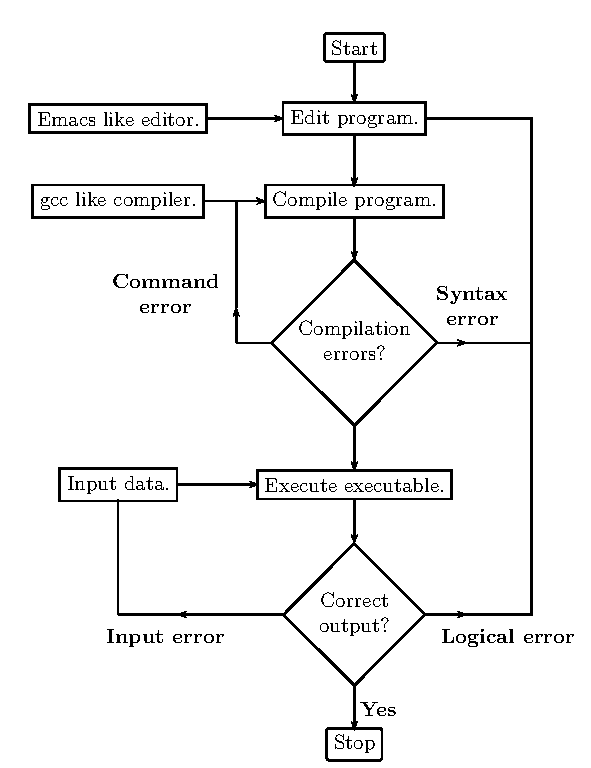
\includegraphics{figs/flowchart-fig1.pdf}
\end{center}
\caption{Life cycle of development of a program}
\end{figure}

\section{Attributes of a Program}
You may be wondering so that is very easy. You just learn programming in C and
start hacking on keyboard to produce software. Well, that is partially true but
a program has several desired attributes which you must consider. Any program
cannot be considered a good program unless it satisfies following requirements
or possess following attributes (Note: These are generic attributes and not
specific to C programming language):
\index{program!attributes}
\begin{enumerate}
\item \textbf{Correctness:}  Correctness means that a program satisfies its
  requirement specification. It means that for a specified input the specified
  output should be produced. This particular attribute is of most
  significance. It does not matter whether other attributes are present or not
  but this one is a must. If a program behavior is not correct then it is of no
  use.
\item \textbf{Efficiency:} Efficiency is second to correctness only. Say you
  are developing a text editor and you take 5 seconds to load a 10KB text file
  then by no means you can persuade a user to use you text editor. A
  program/software must be as efficient as possible. Sometimes it clashes with
  other attributes and also depend on the problem domain that how strict are
  the requirements.
\item \textbf{Security:} A very highly desirable feature in programs which deal
  with more than one computer and also for desktop applications. It is very bad
  if someone can take advantage of buffer overflow, stack overflow, integer
  overflow etc. in your program and you must guard against these at all
  times. Note that to provide security you must put extra checks which will go
  against efficiency.
\item \textbf{Robustness:} Sometimes users will not give correct inputs. For
  example they may enter a character when an integer is asked for or they can
  give input beyond range. In such cases you must handle the erroneous
  input. This is just one example. Sometimes your memory allocation may
  fail. The rule is program defensively. All such input validations and checks
  on memory do take a toll on our second attribute but that does not mean that
  we can neglect it.
\item \textbf{Maintainaibility:} Even a one line program has to be maintained
  if it is worth it! Typically the life of a program far exceeds the
  development time. In almost all the cases the original programmer is not
  maintainer. Because of these reasons you must strive for maintainability. You
  should follow some coding standards like I highly recommend
  \url{http://www.gnu.org/prep/standards/}. Clear documentation is one of the
  prerequisites of maintainability.
\item \textbf{Extensibility:} Let us take our example of text editor and say
  our editor is complete. Now someone else would like to provide a plugin which
  will enable syntax highlighting and project management for this editor. So,
  in order to do so you can choose a plugin-based extensible architecture or
  you can allow them to extend the editor using scripting languages like Guile,
  Python, Lua etc.This features allows user to collaborate and make your
  program better. Remember the rule is the more the merrier here.
\item \textbf{Portability:} It is an elusive and painful but a goal which all
  software desire. Let us say we write our text editor GUI using something like
  Xlib directly then we will have to port the entire GUI for other non X-based
  OSes. So we can choose some cross-platform GUI libraries like GTK+, Qt,
  WxWidgets etc. Even then when system calls come in your software you can do
  not much but either write wrappers and do conditional compilation.
\end{enumerate}

\section{Tools of the Trade}
At the very least you need a compiler, an editor and a linker. Almost all
GNU/Linux systems install GCC by default which is the compiler we are going to
use and it includes linker ld. There are several editors you can use from but I
am going to use Emacs along with Sr-speedbar and Flymake plugins. Other options
include VI, Kate, Gedit, Kwrite etc. A debugger is optional but if you want to
go far with C programming then you must learn to use a debugger. GDB is a very
nice debugger and we are going to use it for debugging in Emacs itself. Emacs
has native support for debugging with GDB. For dynamic memory checking, heap
corruption, cache corruption etc I am going to show you how to use
valgrind. Again, valgrind is optional but it becomes mandatory if you want to
work on large projects. For profiling gprof and for code coverage gcov. Note
that you can use gcc for compiling programs. Most of the GNU/Linux systems come
with gcc. For compiling programs I will use GNU Make though in the beginning I
will show you how to compile on command line. Again, profiling, code coverage
and make are optional to learn C but practically they are necessary to develop
any software worth its value.

You may choose another editor or IDE but I will recommend against IDEs for
beginners as they hide much of compilation process from the users. The reason
of choosing Emacs as an editor is its power. Emacs is hard to learn but it is
very powerful and I implore you to spend some time and learn it. Learning Emacs
will pay rich dividends in future to you. Emacs comes with its manual which you
can read in menu for Help. For using more tools like Sr-speedbar and Flymake
mode you can read more on Emacs Wiki. A lot of extensions are available at
Marmalade Repo. In fact it is wrong to say that Emacs is an editor. You can
read your email, play games, have a shell, read news, do remote editing, browse
web and many other things. It is so powerful that some people set it to run
when they login and they never get out of it.

\section{Bits and Bytes}
\index{bit}
\index{byte}
The smallest unit a computer can understand is called a bit. The term bit 
was coined by John W. Tukey who had also coined ther term software. ``bit'' 
is a contraction for binary digit. His 1958 paper ``The Teaching of Concrete 
Mathematics'' contains the first usage of the word softwrare. The values for a
\index{John Tukey}
bit is either 0 or 1. Consider a voltage. It can be 0V or 1.5V or whatever the
core CPU voltage is. CPU does not understand numbers but voltages :-). You
cannot expect an electronics hardware to understand the same semantics of 0 and
1 which we know. 0 and 1 are abstraction of CPUs voltages in programming. Four
bits form a nibble and eight a byte. A byte is the area of memory which
can be addressed by CPU and its content manipulated. To address a memory a CPU
has say 4 or 8 or up to 256 pins. For example, in a common 32-bit CPU there are
32 pins whose voltages may represent 0 or 1. Consider all pins are low i.e. 0
then the memory location pointed to is 00000000000000000000000000000000 i.e. a
8 bit memory at location 0 can be accessed. This memory is also called primary
memory or RAM (Random Access Memory). So computing this way we can see that a
32-bit processor can access $2^{32}$ bytes or 4,294,967,296 bytes. You can
arrive at this number by 4*1024*1024*1024. This is equivalent to 4GB of
RAM. However, modern Intel processors have 36 physical pins to address up to
64GB of memory. That does not mean that all 64-bit CPUs have 64 pins for
addressing memory as 16 Exabytes(approximately 16 * 10 18 ) is really, really
huge amount of memory which is not needed by any single monolithic system
practically and will be very expensive, thus it is not practical Another point
is that this much memory will require huge area because RAM is not as compact
as hard disk. There are more important practical aspects that if such a
computer fails then it will cause massive loss in productivity of the system
which employs such a computer. Thus computers are kept much smaller than this
size and tasks are divided on those computers and in case one of them fails
then it does not affect the entire system. But all that is an architectural
concern the point I am saying is it is impractical as of now to have so much
RAM in a system but again no one knows future.

Since a byte has 8 bits, its value may range from 0 to 255 as $2^8$ is 256. For
unsigned data type this will be the range. When all bits are 0 value is zero
and when all are high it is 255. Computers use two's complement form to
represent binary number. So if these 8-bits represent signed number the range
will be from $-2^7$ to $2^7-1$ that is -128 to 127. s you will see later at
lowest levels C allows you to access even one bit using something called
bit-fields. If you read specification it will signify the range of one 8-bit
byte as -127 to 127 because it also takes in to consideration of 1’s complement
computers in which positive and negative zeroes are different.

\section{Notes on Number Sytems}
A number system is a system which determines the rules and symbols for numbers
on how we are going to use them. A number system consists of symbols for
representing numbers and a dot for representing fractional numbers. Minus sign
is used to represent negative numbers. A number system ranges from $-\infty$ to
$\infty$. It is best represented by a straight line given below:

\begin{figure}[H]
\begin{center}
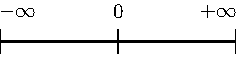
\includegraphics{figs/ns.pdf}
\end{center}
\caption{Number Axis}
\end{figure}

Each point on this axis represents a number. It may be integer or fractional
number. An integer is a whole number like -1, -2, 0, 5, 7 etc. Floating-point
numbers have fractional parts like 1.234. The important fact to note is that
between any two points there exists infinite numbers. In other words between
any two numbers there exists infinite numbers. For example, between 1.2 and 1.3
there are 1.21, 1.22, 1.23..., 1.29. Moreover between 1.21 and 1.22 there are
1.211, 1.212, 1.213 and so on. It enables us to represent a point on this
axis. The numbers I have written are supposedly in decimal number system. Base
of decimal number system is 10. Why because it consists of 10 distinct symbols
0 through 9. Similarly we can have any other number system. Popular number
systems in computers are binary, octal and hexadecimal not to mention decimal
of course.

A number in a generic number system is given below:
\begin{equation}
(.. c_mb^{m-1} + c_{m-1}b^{m-2}+ ... + c_2b^1 + c1_b^0 + c_{-1}b^{-1} +
... + c_{-m}b^{-m} ) \\ = (... c_mc_{m-1}...c_2c_1.c_{-1}...c_{-m})_b
\end{equation}

All the terms with $c$  are called digits. The leftmost or leading digit is
called \textit{most significant digit} and the rightmost or trailing digit is
called \textit{least significant digit}. The . is called a point which
separates the integral part which is towards its left from the fractional part
which is towards its right. $b$  is known as radix or base of the number
system. Note that all digits will be between $0$ to $b-1$. So in our decimal
system $b$  is 10 therefore we have digits from 0 to 9. In binary number system
it is 2 therefore digits permitted are 0 and 1.

\subsection{Binary Number System}
\label{bns}
As the name suggests binary number system has base of 2. Therefore it has only
two symbols. 0 and 1. This is the most popular system for computers because TTL
NAND and NOR gates which are the most basic logic gates using which other gates
are implemented in processor has only two voltage output levels because of
their operation in cut-off and saturation zones. These terms are better
understood with the help of a book on electronics which is out of scope of this
book. All binary numbers consist of 0 and 1. So the count is like 0, 1, 10, 11,
100, 101, 110, 111, 1000 and so on.

\subsubsection{Conversion of Unsigned Decimals and Binaries}
Consider a decimal number. Let us say 53 then how would be convert it to
binary. The technique is that of division. Please examine following carefully:

\hspace*{2cm}
\begin{Verbatim}[frame=single]
  2 | 53 | 1
  ----------
  2 | 26 | 0
  ----------
  2 | 13 | 1
  ----------
  2 | 6  | 0
  ----------
  2 | 3  | 1
  ----------
    | 1  |
\end{Verbatim}

So the binary is $110101_2$. First we divide 53 by 2 and write the
remainder. Then quotient is 26. We repeat the process for 26 therefore
remainder is 0 and quotient is 13. This we go on repeating till we have 1 as
quotient. Note that all the remainders will be 0 or 1 because divisor is
2. Similarly, final quotient is always 1. Now we take final quotient and start
writing remainders from top to bottom.

To convert binary to decimal let us examine following:

$1*2^5 +1*2^4 +0*2^3 +1*2^2 +0*2^1 +1*2^0 =53_{10}$

The power is to 2 because 2 is the base of source. It starts from 0 for unit's
position and increases to 1 and 2 for ten's and hundred's position and so
on. 1's and 0's are the values of that place. If you note carefully powers of 2
grow like 1, 2, 4, 8, 16, 32, 64, 128 and so on. Any number can be written by
using these powers at most one time. For example consider 100. I know it is
less than 128 so I will use 64. Then 36 remains. So I will use 32 and then
4. This means 100=64+32+4  which means power 6, 5 and 2 have been
used. Therefore, I can quickly write down number as $1100100_2$.

\label{fractional binary numbers}
Fractional numbers are slightly more complicated. Let us consider $1.1_2$  . In
decimal it will be $1+\frac{1}{2}$. This is 1.5 in decimal. Note that when you
convert a fractional part of binary to decimal denominator will always be power
of 2. For that matter when you convert from any base to decimal denominator
will be powers of that base. \textbf{Important:} Therefore, when you convert
from decimal to some base n then denominator of that decimal number can have
only those prime factors which are available in the set of prime factors of
$n$.

Let us say we have a fractional number in decimal .59 then to convert it to
decimal we multiply it with 2 which yields 1.018 which is greater than 1 so our
equivalent binary number is .1. Now we subtract 1 from 1.18 to get .18 which
is less than 1 so we multiply it with 2 again to get .36. Now since this is
less than 1 our equivalent binary number is .10. Repeating the process we get
.72 and .100 then 1.44 and .1001. We put 1 in binary part because decimal part
has become greater than 1. Now again we subtract 1 from decimal part to get .44
and repeat the process.

Operations such as addition, subtraction, multiplication and division are
similar in all number systems.

\subsection{2's Complement and 1's Complement}
2's complement and 1's complement are used to convert binary numbers to decimal
values. In 1's complement the number is obtained by inverting bits i.e. making
0 bit to 1 bit and 1 bit to 0 bit of the binary number in question.

Consider the following table which contains some numbers for 1's complement
of some 8-bit numbers.

The 2's complement of an $N$-bit number is defined as the complement with
respect to $2^N$; i.e. it is the result of subtracting the number
from $2^N$, which in binary is one followed by $N$ zeroes. This is also
equivalent to taking the 1's complement and then adding one, since the sum of
a number and its 1's complement is all 1 bits.



%\begin{table}[!bp]
 \begin{center}
\begin{longtable}{|c|r|r|}
\hline
\textbf{Bits}&\textbf{Unsigned Value}&\textbf{1's Complement Value}\\
\hline
0111 1111&127&127\\
\hline
0111 1110&126&126\\
\hline
0000 0010&2&2\\
\hline
0000 0001&1&1\\
\hline
0000 0000&0&0\\
\hline
1111 1111&255&-0\\
\hline
1111 1110&254&-1\\
\hline
1000 0010&130&-125\\
\hline
1000 0001&129&-126\\
\hline
1000 0000&128&-127\\
\hline
 \caption{8-bit 1's complement integers}
\end{longtable}
\end{center}
%\end{table}

For signed numbers MSB(most significant bit) decides sign in both 1's
complement as well as 2's complement. 1's complement has two zeroes. Positive
and negative. As you see in table that 1111 1111 is -0 because MSB is 1 so it
is a negative number and then if you invert all remaining bits then it turns
out to be 0. In a 1's complement system negative numbers are represented by the
arithmetic negative of the value. An $N$-bit 1's complement number system can
represent integers in the range $-2^{N-1} - 1$ to $-2^{N-1} - 1$.

Now it is easy to do addition, subtraction, multiplication, division and other
arithmetic operations. Subtraction for 1's complement is a bit
different. Consider the following:

\begin{Verbatim}[frame=single]
  0000 0110       6
- 0001 0011      19
  ===========   ====
1 1111 0011     -12    -An end-around borrow is produced, and the sign bit
                        of the intermediate result is 1.
- 0000 0001       1    -Subtract the end-around borrow from the result.
  ===========   ====
  1111 0010     -13    -The correct result (6 - 19 = -13)
\end{Verbatim}

Borrows are propagated to the left. If the borrow extends past the end then it
is said to have ``wrapped around'', a condition called an ``end-around
borrow''. When this occurs, the bit must be subtracted from the right-most bit
or least significant bit(LSB). This does not occur in 2's complement arithmetic.

As you see in table and also you can verify the value becomes negative if its
1's complement is computed. However, 2's complement is used on most of
computers because of two zeroes in 1's complement, borrowing being complicated
etc. 

Consider following table of 2's complement 3-bit binary numbers:

%\begin{table}[H]
  \begin{center}
    \begin{longtable}{|c|r|r|}
      \hline
      \textbf{Bits}&\textbf{Unsigned value}&\textbf{2's complement value}\\
      \hline
      011&3&3\\
      \hline
      010&2&2\\
      \hline
      001&1&1\\
      \hline
      000&0&0\\
      \hline
      111&7&-1\\
      \hline
      110&6&-2\\
      \hline
      101&5&-3\\
      \hline
      100&4&-4\\
      \hline
    \caption{3-bit 2's complement integers}
    \end{longtable}
  \end{center}
%\end{table}
Clearly, since $N$-bit 1's complement can represent numbers in range
$-2^{N-1}-1$ to $2^{N-1} + 1$ 2's complement of $N$-bit can represent
$-2^{N-1}$ to $2^{N-1} - 1$ as it does not have negative 0 i.e. its range is
more by 1 number.

The 2' complement system has the advantage that operations of addition,
subtraction, and multiplication are same as unsigned binary numbers (as long as
the inputs are represented in the same number of bits and any overflow beyond
those bits is discarded from the result). This property makes the system both
simpler to implement and capable of easily handling higher precision
arithmetic. Also, as mentioned above zero has only a single 
representation, avoiding the subtleties associated with negative zero, which
exists in 1's complement systems.

The value $v$ of an $N$-bit integer $b_{N-1} b_{N-2} \dots b_0 $is given by the
following formula:

\begin{equation}
v=-b_{N-1} 2^{N-1} + \sum_{i=0}^{N-2} b_i 2^i
\end{equation}

I will leave it up to you, the reader, to perform basic operations like
addition, subtraction, multiplication, division etc.

\section{Compiling and Executing}
\index{program!compilation}
\index{program!execution}
To compile and execute a program create a new file, edit it and save it. The
extension of file should be \texttt{*.c}. For example,
\texttt{myprogram.c}. After that you can give this command at terminal. Here is
the corrected code.

\begin{minted}[frame=single]{c}
#include <stdio.h>

int main()
{
  return 0;
}
\end{minted}

Execute the following command on your command prompt:
\\\\\$gcc nothing.c -o nothing\\\\
Here \texttt{nothing.c} is the name of the file with which it was saved.

Then you will see a file named my program is created by compiler if no errors
were there in your program. In case of errors, like we had in one shown to you
they have to be resolved first. Executable \texttt{nothing} is produced then
you can execute it like
\\\\\$./nothing\\\\
Note that in both the commands \texttt{\$} is not part of command but it is
prompt. For you it may be \texttt{\%} or \texttt{\#} or something fancier
(depends on the imagination of your system administrator). To execute this
command your working directory must be same as the directory your program is
in.

\color{nicered}
\dangersign[3ex] Also, note that on some systems \texttt{TAB} auto completes filename so do
not do the following by accident:
\\\\\$gcc nothing.c -o nothing.c\\\\
\color{black}
This will overwrite your \texttt{nothing.c} by the result of compilation binary
with the same name \texttt{nothing.c}. Let us see how to compile this program
using a Makefile. Edit your \texttt{Makefile} like this:

\begin{minted}[frame=single]{makefile}
#sample Makefile
check-syntax:
    gcc -o nul -Wall -S $(CHK_SOURCES)

nothing: nothing.c
    gcc -Wall -std=c11 -pedantic nothing.c -o nothing
\end{minted}

Now from do this from menu. \texttt{Tools->compile} As the command issue
\texttt{make -k test}. Another way to do the same using keyboard only is type
\texttt{M-x compile} and repeat \texttt{make -k test} as previous time. Your
code will be compiled. Makefiles are better than executing commands 
repeatedly again and again however you must know underlying commands. I will
discuss the compiler options as appropriate. \texttt{-Wall} will enable all the
warnings from \texttt{gcc}, \texttt{-std=c11} enables new features of C11
standard and \texttt{-pedantic} ensures specification conformance. 

So let us get started with basics of C.

%\chapter{Basics of C}
There are certain rules in every language, certain grammar which dictates the
way language will be spoken and written. It has a script to write
using. Similarly, programming languages have BNF (Backus-Naur Form)
context-free grammar. There are valid characters in a programming language and
a set of keywords. There are constructs to handle control flow, loops
etc. There are facilities provided by language to deal with numbers and strings
separately, to reuse the code and some basic data structures to facilitate
programming. However, programming language ruleset is very small compared
to a natural programming language. Also, when using natural programming
language like talking to someone or writing something the other person can
understand your intent but in programming you cannot violate rules. The grammar
is context-free. Compilers or interpreters cannot deduce your intent by reading
code. They are not intelligent. You make a mistake and it will refuse to listen
to you no matter what you do. Therefore, it is very essential to understand
these rules very clearly and correctly.

\section{The C Character Set}
The following form the C character set you are allowed to use in it:

\begin{verbatim}
[a-z] [A-Z] [0-9] ~ ! # % ^ & * ( ) - = [ ] \ ; ' , . / _ + { } | : " < > ?
\end{verbatim}
\index{character set}

This means along with other symbols you can use all English alphabets (both
uppercase and lowercase) and Arabic numerals. Symbols like \texttt{\$} and
\texttt{@} are not part of C's character set. But strings can contain any
these characters also. Strings are sequence of characters with double quotes
and double quotes iteself are escaped with \texttt{$\backslash$}. Also,
\texttt{\$} and \texttt{@} can also be value of characters. Characters are
values containing single characters withing single quotes. We will see more of
these in their individual sections. However, English is not the only
spoken language in the world. Therefore in other non-English speaking counties
there are keyboard where certain characters present in above set are not
present. The inventors of C were wise enough to envision this and provide the
facility in form of trigraph sequences. Given below is the trigraph sequence
table:

\begin{table}
 \begin{center}
 \caption{Trigraph Sequences}
\begin{tabular}{|c|c|c|c|c|c|}
\hline
\textbf{Trigraph}&\textbf{Equivalent}&\textbf{Trigraph}&\textbf{Equivalent}&\textbf{Trigraph}&\textbf{Equivalent}\\
\hline
??=&\#&??'&\textasciicircum&??!&|\\
\hline
??(&[&??)&]&??$<$&\{\\
\hline
??$>$&\}&??/&\textbackslash&??-&\textasciitilde\\
\hline
\end{tabular}
\end{center}
\end{table}
\index{trigraph sequences}

However, you should refrain from using trigraph sequences for portability 
reasons as suggested by GNU coding standards.

\section{Keywords}
The following are reserved keywords for C programming language which you are not 
allows to use other than what they are meant for:
\index{keywords}
\begin{table}[H]
 \begin{center}
  \caption{Keywords of C}
  \begin{tabular}{l l l l l}
    auto & break & case & char & const\\
    continue & default & do & double & else\\
    enum & extern & float & for & goto\\
    if & inline & int & long & register\\
    restricted & return & short & signed & sizeof\\
    static & struct & switch & typedef  & union\\
    unsigned & void & volatile & while & \_Bool\\
    \_Complex & \_Imaginary & &\\
  \end{tabular}
 \end{center}
\end{table}

These keywords are special in C as said and cannot be used for variable names 
or funciton names or otherwise other than in strings and comments.

\section{Identifiers}
The names which we give to our variables are known as identifiers. Something 
with which we identify the variables. As you have already seen what is allowed 
in C's character set but not all are allowed in an identifiers name. Only 
alphabets from English language both lowercase and uppercase, Arabic digits from 
zero to nine and underscore (\_) are allowed in an identifiers name. The rule 
for constructing names is that among the allowed characters it can only begin 
with only English alphabets and underscore. Numbers must not be first character. 
For example, \texttt{x, \_myVar, varX} and \texttt{yourId78} are all valid 
names. However, take care with names starting from underscore as they are mostly 
used by different library authors. Invalid identifier examples are \texttt{9x, 
my\$} and \texttt{your age}. Please read this section carefully and make sure 
understand the rules for naming identifiers. Later at the end of chapter there 
are some simple problems to practice with.

\section{Programming}
Let us revisit our first program and try to understand what it does. Here I am 
giving code once again for quick reference:

\begin{minted}{c}
// My first program
/* Description: This program does nothing.*/

#include <stdio.h>

int main(int argc, char* argv[])
{
  return 0;
}
\end{minted}

You can now issue a command as \texttt{\$gcc nothing.c} where 
\texttt{nothing.c} is the filename by which you saved the source code. Note 
that \texttt{\$} is the prompt not part of command itself. Then you can do an 
ls and you will find that \texttt{a.out} is a file which has been produced by 
clang. Now you can run this program by saying \texttt{\$./a.out} and nothing 
will happen. But if you type \texttt{\$echo \$?} then you will find that 0 is 
printed on screen which is nothing but 0 after \texttt{return} of our program.

As you can see this program does almost nothing but it is fairly complete 
program and we can learn a lot from it about C. Let us try to dissect it line
by line. The first line is a comment. 
Whenever C compiler parses C programs and it encounters \texttt{//} it ignores 
rest of line as code i.e. it does not compile them. This type of single line 
comment were introduced in C99 standard and if your compiler is really old the 
compiler may give you error message about it. The second line is
also comments. Anything between \texttt{/*} and \texttt{*/} is ignored like 
\texttt{//}. However, be careful of something like \texttt{/* some comment */
  more comment */}. Such comments will produce error messages and your program
will fail to compile. The reason for this is when first \texttt{*/} is
encountered by parser or compiler it will complete its token for the comment
and then further portion which we intented to be part of comment will cause
syntax error. 

Comments are very integral part of programming. They are used to describe 
various things. You can write whatever you want. They may also be used to 
generate documentation with tools like doxygen. Typically comments should tell
what the program is doing not how. Sometimes how can be covered, when the logic
is really complex. One should be generous while commenting the code.

The next line is \texttt{\#include <stdio.h>}. \texttt{\#include} is a
preprocessor directive. The preprocessor directive is handled by the C
preprocesor which is handled by C preprocessor which looks in four directories
for include files. The include filename comes after \texttt{\#include} either in
angular brackets or double quotes. The C preprocessor looks for these at four
different places at least out of which one or posiibly two is of interest for
now as we are dealing with angular brackets. Depending on the way your compiler
is installed the file \texttt{stdio.h} may be in \texttt{/usr/include} or
\texttt{/usr/local/include} but then again it may be in a non-standard path
also although possibility of that is very less and then it is controlled by
parameters whose discussion is beyond the scope of book. Let us say
\texttt{stdio.h} is present in either of aforementioned directories then the C
preprocessor will copies the contents and pastes them in source file along the
way putting \texttt{\#line} macros which are used for debugging
purposes. \texttt{\#line} macro is discussed later in the chapter which deals
with macros. You can see the output of C preprocessor by typing \texttt{\$gcc
  -E nothing.c} since it will scroll a lot on you terminal you can use a pager
like \texttt{less} to read it. The \texttt{-E} tells \texttt{gcc} to just allow
preprocessoing and not compile and link the file.

I have recorded a video on basics of compilation which you can see at
\url{http://www.youtube.com/watch?v=ARsoVgknRU0}.

Next line is \texttt{int main(int argc, char* argv[])}. Now this is very special
function. Every complete executable(shared objects or dlls or archive
libraririe do not have main even though they are C programs) C program will
have one main function unless you do assembly hacking. This function is where
the programs start. The first word \texttt{int} is a keyword which shirthand
for integer. This signifies the return type of function. \texttt{main} is the
name of the function. Inside parenthesis you see \texttt{int argc} which tells
how many arguments were passed to program and is short form of argument
count. While \texttt{char* argv[]} is a pointer to array which we will see
later. For now let us just remember that it holds all the arguments to the
program including the program name.

Next is a brace. The scope in C is determined by braces. Something outside any
brace has global scope (we will see these later), something inside first level
of brace has function or local scope. Something inside second or more level of
braces have got that particular block scope. Scope here means that when there
will be a closing brace that particular variable which is valid in that scope
will cease to exist. However, we do not have to worry about that yet as we do
not have any variable. Just note that a corresponding closing brace will be the
end of main function. For every opening brace which starts a scope a closing
brace is mandatory.

Next line is \texttt{return 0;} This means whoever has called \texttt{main()}
will get a 0 as \texttt{return} is returning 0. In this case, receiver is the
shell or operating system 
which has invoked the very program. The semicolon is called the terminator and
used also on Java or C++ for example. The very requirement of semicolon is to
terminate the statement and move on to next statement.

However, the program shown does not do much. Let us write a program which has
some more functionality and we can explore more of C. So here is a program
which takes two integers as input from users and presents their sum as
output. Here is the program:

\begin{minted}{c}
// My second program
// Author: Shiv S. Dayal
// Description: It adds two numbers

#include <stdio.h>

int main()
{
  int x=0, y=0, sum=0;

  printf("Please enter an integer:\n");
  scanf("%d", &x);

  printf("Please enter another integer:\n");
  scanf("%d", &y);

  sum = x + y;

  printf("%d + %d = %d\n", x, y, sum);

  return 0;
}
\end{minted}
and the output is:
\begin{verbatim}
shiv@shiv:~/book/code$ ./addition
Please enter an integer:
7
Please enter another integer:
8
7 + 8 = 15
shiv@shiv:~/book/code$
\end{verbatim}

Note that \texttt{shiv@shiv:~/book/code\$} is the prompt.

Let us discuss new lines one by one. The line \texttt{int x=0, y=0, z=0;} is
declaration and definition or initialization of three ints. \texttt{int}
keyword in C is used to represent integers. Now we have three integers with
there values set to 0. Note that how the variables are separated by commas and
terminated by semicolon(as we saw in last program also). We could have also
written it like this:

\begin{minted}{c}
int x;
int y;
int z;

x = 0;
y = 0;
z = 0;
\end{minted}

or

\begin{minted}{c}
int x, y, z;

x = y = z = 0;
\end{minted}

However, the first method is best and most preferred as it prevents use before
definition. \texttt{int} is a data-type in C. \texttt{x, y,} and \texttt{z} are
called variables of type \texttt{int}. This means that the size of these
variables will be same as \texttt{int}. Note that 
C is a statically typed language and all types have predefined memory
requirements. In cour case, \texttt{int} requires 4 bytes on 32-bit and 64-bit
systems but 2 bytes on 16-bit systems.

Here I have created a video about variables of C which you can see at
\url{http://www.youtube.com/watch?feature=player\_embedded\&v=6whuGZwv2-k} and
you can watch another about \texttt{printf} and \texttt{scanf} at
\url{http://www.youtube.com/watch?feature=player\_embedded\&v=U3jCSTR7Ulo}.

Let us learn a bit about \texttt{printf}. This function is declared in
stdio.h. The prototype of \texttt{printf()} is

\begin{minted}{c}
int printf(const char *restrict format, ...);
\end{minted}

The first argument format is what we have in first two function calls. The
second is a \texttt{...} which means it can take variable number of arguments
known as variable-list. We have seen this in the third call.This means it will
take a string with optional variable no. of arguments. The string is called the
format-string and determines what can be printed with supplied arguments. These
\texttt{...} are used to supply variable no. of arguments. In the first two
\texttt{printf()} statements we just print the format-string so that is
simple. However, in the last one, we have format as \texttt{\%d} which
signifies a decimal integer. The integers printed are in the same order in
which they were supplied.

\texttt{scanf()} is scan function which scans for keyboard input. As by now you
know that \texttt{\%d} is for decimal integer but we have not said \texttt{x}
or \texttt{y}. The reason is \texttt{x} and \texttt{y} are values while
\texttt{\&x} and \texttt{\&y} are the addresses of \texttt{x} and \texttt{y} in
memory. \texttt{scanf()} needs the memory address to which it can write the
contents to. You will see \texttt{\&} operator in action later when we deal
with pointers. Just remember for now that to use a simple variable with
\texttt{scanf()} requires \texttt{\&} before its name.

Till now we have just seen only \texttt{int} data-type but then there are more
data types for other types of numbers, characters and strings. Let us see them
one by one.

\section{Data Types}
What are data types? Why C needs data types? C is a statically typed language
that is every variable has a type associated with it. These types determine
what kind of values these variables can hold and how they will be interpreted.
When everything is a voltage level why not just deal with 0s and 1s? The answer
is simple. You need to abstract and segregate how much is required. For
example, say you are given a sequence of 0s and 1s how much can you work with
them. We as humans are not very versed with 0s and 1s. Also, say we encode
character `A' for 10101 will it be easy for you to see A or numbers. Also,
numbers range from $-\infty$ to $\infty$. Also, since C is statically typed the
sizes of data types have to be known at compile time. There are four types of
data types. Integral, floating-point, arrays and pointers. Here, I will deal
with the two former types and leave latter two for later. The integral types
are \texttt{char, short int, int, long} and \texttt{long long} and
floating-point types are \texttt{float, double} and \texttt{long
  double}. \texttt{signed} and \texttt{unsigned} are sign modifiers which also
modified the range of data types but do not affect their memory
requirements. By default all basic data types are \texttt{signed} in nature and
you must qualify you variables with \texttt{unsigned} if you want that
behavior. \texttt{short} and \texttt{long} are modifiers for size which the
data type occupies but I consider them as different types because memory
requirements are different. The ranges of integral data types directly reflect
their memory requirements and if you know how much memory they are going to
occupy you can easily compute their ranges. The range of floating-point comes
from IEEE specification. IEEE standard document 754 governs the binary
representation of floating point numbers which you can read at
\url{http://www.eecs.berkeley.edu/~wkahan/ieee754status/IEEE754.PDF}. This is
not available from IEEE website itself as they sell the specification's
electronic copies.

Let us write a program to find out ranges for integral data types:

\begin{minted}{c}
// Description: It gives ranges of integral data types

#include <stdio.h>
#include <limits.h>

int main()
{
  printf("Size of char is..........%d\n", sizeof(char));
  printf("Size of short int is.....%d\n", sizeof(short int));
  printf("Size of int is...........%d\n", sizeof(int));
  printf("Size of long is..........%d\n", sizeof(long));
  printf("Size of long long is.....%d\n", sizeof(long long));
  printf("Size of float is.........%d\n", sizeof(float));
  printf("Size of double is........%d\n", sizeof(double));
  printf("Size of long double is...%d\n", sizeof(long double));c

  return 0;
}
\end{minted}

Here \texttt{sizeof} is a compile time operator which computes size of any type
passed to it as an argument. So it is computing sizes of all the data types as
shown in the program. The output is given below:

\begin{verbatim}
Size of char is..........1
Size of short int is.....2
Size of int is...........4
Size of long is..........8
Size of long long is.....8
Size of float is.........4
Size of double is........8
Size of long double is...16
\end{verbatim}

Please note that the output shown is on 64-bit machine and it will be different
on 32-bit machines.
%\chapter{Console I/O}
IO stands for input/output. C provides only mechanism to interact through
console using its standard library. C does not provide ways to have GUI
although that is possible with various GUI libraries most notable being
GTK. However, discussing about GTK is out of scope of this book. In this
chapter we will focus on console output facilities of C because any program we
write at this stage will be meaningless if it has no input/output. Typically
when we interact with a C program we give input using keyboard which is also
referred as \texttt{stdin} stream. The output is monitor or \texttt{stdout}
stream. There is one more stream \texttt{stderr} which is generally redirected
to monitor or a log file. For historical reasons these are known as
\texttt{FILE} stream which represents the datatype of these
streams. \texttt{FILE} is capable of representing other streams which are disk
based for example a file on your hard drive. There are more type of input
devices on a modern computer. For example, network i/o is there. Whenever you
browse web or download a file through your intenet connection network i/o comes
into play. There is an opengroup
which specifies functions for network related functions. Operating systems
like GNU/Linux are POSIX compatible which defines how network i/o will be
used. Even a printer is a special output device, a camera input, speakers
output, microphone input and so on. In this books we are concerned with
keyboard input, output on monitor and i/o using files. Other types of i/os are
out of scope of this book.

However, before we go on with i/o I would
like to present C's memory model which will be needed by our discussion of i/o
related functions. However, if things do not make sense even then please go
through it and come later to understand more. 

\section{C's Memory Model}
As you may be knowing RAM(random acess memory) is the area which is used as
primary memory. Whenever we execute a program the first thing which happens is
that it gets loaded into memory. Now a binary program becomes a process when it
is running i.e. a running program is referred as process. All processes have
memory area divided into different portions. These portions are known as data
segment, stack and code or text segment. Dats segement is further split in
three parts; initialized data segment, uninitialized data segment or BSS which
is name after an ancient assembler Block Started by Symbol and
heap. Initialized data segment contains initialized global variables and static
variables. For uninitialized data segment it is same as above just that the
variables are not initialized explicitly but implicitly to zero.

Heap is the largest area of memory used for dynamic memory allocation. As
you will see later that you can manage heap using \texttt{malloc(), calloc(),
realloc(),} and \texttt{free()}. Note that operating system does not manage memory
allocated for you on heap. You, the programmer, are responsible for allocating and
freeing up memory in area. If heap gets full os will use virtual memory or swap
space on hard disk. Objects allocated on heap persist across function
calls. However, there are some very nasty problems, which, come in picture when
you use heap. There are several of them. You may forget to allocate memory and
may dereference unallocated pointer. You may have initialized it to
\texttt{NULL} and try to dereference that. You may allocate and free twice. You
forgot to set pointer to \texttt{NULL} after freeing it. And last but not the
least you loose all pointers to the memory area before you can free. The nature
with this particular problem is that if your program is going to run for long
time then it is going to consume more and more memory. Because of its nature it
is known as memory leak. It is very difficult to detect such problems in code
which does not run for long periods of time. Our friend valgrind will come to
help up with this problem. When a memory leak happens it eats up RAM slowly and
then operating system has to use virtual memory as explained above. In a
nutshell, I will say that heap means you have to manage it.

\begin{figure}[t!]
\begin{center}
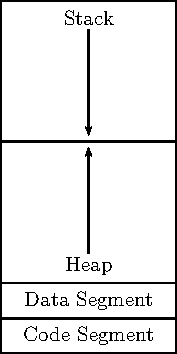
\includegraphics{figs/mem_model.pdf}
\end{center}
\caption{Memory model of a C program}
\end{figure}

Stack is relatively simple. All non-static and non-register variables go on
stack if not allocated dynamically. Stack variables do not retain there value
across function calls unless
they are passed as pointers. Also, when they go out of
scope, that is the scope in which they were declared ends, they will be kind of
lost. The way in which stack frame moves the same area will be used for new
variables. However, stack is very limited (compared to heap) and in deeply
nested function calls or recursion (you will see these in Functions chapter)
stack may get full and program may crash. The reason for crashing is that
operating system will not use virtual memory but will do a segmentation fault
in its place. GNU/Linux allow its users to modify the stack size by ulimit
command. Note that stack and heap are adjacent in memory and grow in opposite
direction.

Code segment or text segment is an area where the executable instructions of
program reside. It is typically constant and read-only area unless your system
allows self-modifying code. Following diagram shows the memory layout.

Note that this memory model not only applies to C but any process.

Now we will look at those functions, which, allow us to do console i/o. We will
begin with our familiar friends; printf and scanf.

\section{printf}
The prototype of \texttt{printf} is given by

\begin{Verbatim}[frame=single]
int printf(const char* fmt, ...);
\end{Verbatim}

Let us take a minute to understand this as we have not yet covered
functions. The first word is \texttt{int} which denotes the return type of the
\texttt{printf} function. This is no. of characters printed. Then we have name
of the function. \texttt{fmt} is the format string of type \texttt{const
 char}. In C, strings are either character arrays or character pointers. Here,
const means \texttt{printf} will not modify the format string. The ... means
variable no. of arguments, which, can be 0 also to be supplied to
\texttt{printf}.

\texttt{printf} is a string based output function that is It writes character
strings to \texttt{stdout}. The data which has to be written is formatted by
format string as shown previously. After the format specifier it expects as
many arguments as specified in format string. The characters which are not
like, say \texttt{\%d} for example, arecalled ordinary characters. These are
simply copied to output stream, which, is stdout for printf. The \texttt{\%d}
like conversion charcaters are known as conversion specification or format
specifiers. Each conversion specification should be augmented with one one
argument. The results are undefined if there are insufficient arguments for the
format. If extra arguments are given the excess arguments will be evaluated but
are otherwise ignored. However, there is a big problem here! There is no
type-safety. In general compiler will warn you about it and you, the
programmer, are responsible for giving correct format string, correct no. of
correct type of arguments. Consider the following program for example:

\begin{Verbatim}[frame=single]
#include <stdio.h>

int main()
{
  printf("%d %d\n", 3, 8);

  //do not mess it. undefined behavior
  printf("%d %d\n", 5);

  //extra arguments ignored
  printf("%d %d\n", 3, 5, "hello");

  //legal because char is integer type
  printf("%d\n", 's');

  //wrap around of integer as char
  printf("%c\n", 836);

  //do not mess with type-safety
  int i = printf("%d\n", "hello");
  prinf("%d\n", i);

  return 0;
}
\end{Verbatim}

now that if you give the command like \texttt{gcc -Wall printf.c} where
\texttt{printf.c} is the name of the ile then you will be shown following
warnings:

\begin{Verbatim}[frame=single]
printf.c: In function 'main':
printf.c:8:3: warning: format '%d' expects a matching 'int' argument [-Wformat=]
   printf("%d %d\n", 5);
   ^
printf.c:8:3: warning: format '%d' expects a matching 'int' argument [-Wformat=]
printf.c:11:3: warning: too many arguments for format [-Wformat-extra-args]
   printf("%d %d\n", 3, 5, "hello");
   ^
printf.c:11:3: warning: too many arguments for format [-Wformat-extra-args]
printf.c:20:3: warning: format '%d' expects argument of type 'int', but
argument 2 has type 'char *' [-Wformat=]
   int i = printf("%d\n", "hello");
   ^
printf.c:20:3: warning: format '%d' expects argument of type 'int', but
argument 2 has type 'char *' [-Wformat=]
\end{Verbatim}

Clearly this is not a good sign for any program. A program should compile
cleanly. In our case \texttt{gcc} is generating binary even though there are
warnings. You can make \texttt{gcc} generate more warnings by issuing a
\texttt{-Wall} flag. You can also treat all warnings as errors by passing
\texttt{-Werror} to \texttt{gcc}. These two options will ensure that your code
has no warnings. Now let us move to output and try to understand it. The output
on my system is as given below. It may differ on your system:
\\\\\texttt{3 8\\
5 8\\
3 5\\
115\\
D\\
134514119\\
10\\\\}
First \texttt{printf} is correct as expected. The second line causes undefined
behavior. You may think it is the previous 8 but believe me it is not
guaranteed that it will always the case. Ii is \textbf{UNDEFINED}. Third
\texttt{printf} is also fine in the sense that extra argument is
ignored. Fourth and fifth are normal. Sixth is again a big problem. You are
trying to print a decimal integer while argument is a character string. There
is no way for compiler to determine that what should be printed which will fit
on standards.

A full detail of all conversion specification is given in specification at \S(iso.7.21.6).

In real-world most of the time the conversion specifiers are kept simple. Given
below is a sample program showing some of the things given above:

\begin{Verbatim}[frame=single]
#include<stdio.h>

int main()
{
  int i   = 343456;
  float f = 123;
  long double ld = 78939.9347;

  printf("% d\n", i);
  printf("%+d\n", i);
  printf("%#o\n", i);
  printf("%#f\n", f);
  printf("%-08i\n", i);
  printf("%08i\n", i);
  printf("%8i\n", i);
  printf("%hhi\n", i);
  printf("%hi\n", i);
  printf("%li\n", i);
  printf("%lli\n", i);
  printf("%ji\n", i);
  printf("%zi\n", i);
  printf("%ti\n", i);
  printf("%8.8f\n", f);
  printf("%8.8Lf\n", ld);

  return 0;
}
\end{Verbatim}

The output of the above program is:
\\\\\texttt{ 343456\\
+343456\\
01236640\\
123.000000\\
343456\\
00343456\\
  343456\\
-96\\
15776\\
343456\\
4638355772471066016\\
4638355772471066016\\
343456\\
343456\\
123.00000000\\
78939.93470000\\\\}
We will keep seeing more conversion specifiers being used as we progress
through this book.

\section{scanf}
It scans \texttt{stdin} or keyboard for input. Its signature is same as that of
\texttt{printf()}. It reads bytes from keyboard input, interprets them
according to format string. It also expects a set of pointer arguments as
opposed to values for printf(). The pointers indicate where the interpreted
data from the input will be stored. The result is \texttt{UNDEFINED} if there
are less number of pointer arguments than the number of conversion specifers in
format string. Excess arguments will be evaluated but ignored. The format
string can have only white-space characters or an ordinary character (neither
`\%' nor a white-space character) or a conversion specification. Each
conversion specification is introduced by `\%', after which the following
appear in sequence.

For now if you do not understand what is a pointer then let us have a simple
definition for that. A pointer is a variable which stores a memory location
where the value will be stored.

Now that we have seen this description let us take a look at few examples.

\begin{Verbatim}[frame=single]
#include <stdio.h>

int main()
{
  char str[128] = {0};

  scanf("%s", str);
  printf("You entered:\n%s\n", str);

  return 0;
}
\end{Verbatim}

and the output is:
\\\\\texttt{\textbf{Hi! My name is Shiv.\\}
You entered:\\
Hi!\\\\}
It is certainly not the correct output. We had expected to see like: ``Hi! My
name is Shiv.''. What happend to input string after ``Hi!''. Well, in a form
given above for \texttt{scanf()} it will stop taking input after white-space
for character strings. For numerics it does not matter as it does not match the
format. For characters it is character-by-character so no confusion either. So
what if you want to have the entire string including white-spaces. Use
\texttt{[\^{}n]} as given below:

\begin{Verbatim}[frame=single]
#include <stdio.h>

int main()
{
  char str[128] = {0};

  scanf("%[^\n]s", str);
  printf("You entered:\n%s\n", str);

  return 0;
}
\end{Verbatim}

and the output is:
\\\\\texttt{\textbf{Hi! My name is Shiv.}\\
You entered:\\
Hi! My name is Shiv.\\\\}
What if you want to filter a string based on certain patterns. For example, a
charcater string does not contain more that a single space, English alphabets,
period and digits. To scan such a string you can define a pttern as program
given below shows:

\begin{Verbatim}[frame=single]
#include <stdio.h>

int main()
{
  char c[100]={0};

  scanf("%[ A-Za-z0-9!.]", c);
  printf("%s\n", c);

  return 0;
}
\end{Verbatim}

and the output is:
\\\\\texttt{\textbf{Hi! My name is Shiv! My phone no. is 1234. \%\^\$\&\*\\}
Hi! My name is Shiv! My phone no. is 1234.\\\\}
There is also a major problem associated with input and that comes when you
have characters involved. Consider the following program:

\begin{Verbatim}[frame=single]
#include <stdio.h>

int main()
{
  int   i = 0;
  float f = 0.0;
  char  c1 = '\0';
  char  c2 = '\0';
  char  c3 = '\0';

  printf("Enter an integer, a float and three character one by one:\n");

  scanf("%d", &i);
  scanf("%f", &f);
  scanf("%c", &c1);
  scanf("%c", &c2);
  scanf("%c", &c3);

  printf("You entered\n");
  printf("%d\n", i);
  printf("%f\n", f);
  printf("%c\n", c1);
  printf("%c\n", c2);
  printf("%c\n", c3);

  return 0;
}
\end{Verbatim}

and the output is:
\\\\\texttt{\textbf{2\\
3.4\\
s\\}
You entered\\
2\\
3.400000\\
\\
\\
s\\\\}
What is happening here is that newline entered by our RET key is getting
assigned to \texttt{c1} and \texttt{c3}. That is why the program accepted only
second character. The enter after \texttt{float f;} was assigned to \texttt{c1}
and the character entered to \texttt{c2} and then the RET newline to
\texttt{c3}. There is a very simple way to recover from this:

\begin{Verbatim}[frame=single]
#include <stdio.h>

int main()
{
  int   i = 0;
  float f = 0.0;
  char  c1 = '\0';
  char  c2 = '\0';
  char  c3 = '\0';

  printf("Enter an integer, a float and three character one by one:\n");
  scanf("%d", &i);
  scanf("%f", &f);
  scanf(" %c", &c1);
  scanf(" %c", &c2);
  scanf(" %c", &c3);

  printf("%d\n", i);
  printf("%f\n", f);
  printf("%c\n", c1);
  printf("%c\n", c2);
  printf("%c\n", c3);

  return 0;
}
\end{Verbatim}

The whitespace character shown will eat up all the white-space given after the
previous input. This concludes our discussion on \texttt{printf()} and
\texttt{scanf()}. Now we will move to another set of i/o functions which take
character string without filtering and print it to screen without
filtering. What I am going to discuss are \texttt{gets(), fgets(), puts()} and
\texttt{fputs()}.

All the following function's reference is present in \S(iso.7.21) which deals with
header `stdio.h`.

\section{Sting I/O Functions}
These functions are very simple compared to \texttt{printf(}) and
\texttt{scanf()}. They take a pointer to a character array or a character
pointer and fill it with input or print it to monitor. Note that
\texttt{gets()} and \texttt{puts()} work only with \texttt{stdin} and
\texttt{stdout} respectively while \texttt{fgets()} and \texttt{fputs()} work
with \texttt{FILE} streams i.e. other than \texttt{stdin} and \texttt{stdout}
they can also work with disk based files. Here is a sample program:

\begin{Verbatim}[frame=single]
#include <stdio.h>
#include <stdlib.h>

int main()
{
  char cStack[1024] = "";
  char *cHeap = (char*)malloc(sizeof(1024));

  gets(cStack);
  puts(cStack);

  cHeap = fgets(cHeap, 1024, stdin);
  fputs(cHeap, stdout);

  return 0;
}
\end{Verbatim}

and the output is:
\\\\\texttt{\textbf{Hi!\\}
Hi!\\
\textbf{Hello!\\}
Hello!\\\\}
First \texttt{``Hi!''} and \texttt{``Hello!''} are keyboard inputs. Do not
worry about array and pointer syntax at the moment. Just see the difference
between function calls. Their is a problem with \texttt{gets()} that it can
cause buffer overflow. If input is bigger than 1024 bytes including the null
terminator then buffer overflow will happen. Note how you can prevent it with
\texttt{fgets()} by specifying the number of characters you want to read. Rest
of input will be ignored by \texttt{fgets()}. This is a security hole and
therefore you should never ever use \texttt{gets()}.

\section{Character I/O Functions}
There are several functions for single character i/o. They are \texttt{getc(),
  putc(), getchar(), putchar(), fgetc()} and \texttt{fputc()}. Apart from
\texttt{getchar()} and \texttt{putchar()} rest can do any FILE stream-based
i/o. Let us have a simple program as they are mostly trivial.

\begin{Verbatim}[frame=single]
#include<stdio.h>

int main()
{
  char c ='';

  c = getchar();
  putchar(c);

  c = getchar();
  putchar(c);

  c = fgetc(stdin);
  fputc(c, stdout);

  c = getchar();
  putchar(c);

  c = getc(stdin);
  putc(c, stdout);

  return 0;
}
\end{Verbatim}

and the output is:
\\\\\texttt{\textbf{4\\}
4\\
\textbf{5\\}
5\\
\textbf{6\\}
6\\\\}
The first 4, 5 and 6 were keyboard inputs. Note the use of extra
\texttt{getchar()} and \texttt{putchar()} to handle the situation we faced
during \texttt{scanf()}.



%\chapter{Operators and Expressions}
Operators and expressions are in the core of every programming language. They
form the major part of BNF grammar. They also decide how the syntax will look
like. You as a programmer will spend considerable time using C operators. C has
several type of operators like arithmetic operators, relational operators,
bitwise operators, unary operators, logical operators to name some of them.
Since C was first of very popular structured general-purpose languages therefore
many modern language use almost all the operators and supplement with their own.
It is needless to say that to become a good programmer you must know all the
operators of C and know where to use which one as it may decide performance,
readability, simplicity of your code. Whenever you see array and pointer in
following sections just plow through them. All will be clear soon.

Before we can proceed to discuss operators and expressions I will explain
scope, linkage and storage durations which can be applied to
variables. These are given in specification starting in \S(iso.6.2.1) and ending at
\S(iso.6.2.4).

\section{Scope of an Identifier}
Till now we have seen plain variables and their identifiers. However, there are
other identifiers as well which will be discussed later. For now we will
consider scope of plain variables. In general there are three kinds of
scope. Global scope, function scope and block scope. Variables declared outside
any function have global scope and they persist throughout the lifetime of the
program. Variables declared inside functions at outermost level have function
scope and they live as long as function remains active. A block in C is marked
by braces(\{ and \}). Function bodies are also marked by this. Here I mean
blocks inside a function. Starting from C99 you can declare variables anywhere
inside a function and this block variables which have less lifetime than
functions are possible. We will see more of these when we see more code. Note
that identifiers can be reused in different scopes. For example, a loop index
integer identifier is repeated many times but every time it is a new
variable(We will see loops soon). Two identifiers have same scope if and only
if their scope terminates at the same point.

\section{Linkages of an Identifier}
There are three different kinds of linkages. External, internal and
none. Global variables and functions have external linkage as long as they are
not static. If they are static then they have internal linkage. By external
linkage we mean that for a program which consists of multiple source code files
these functions and variable identifiers can be referred in files other than in
which they are declared. When functions and global variables are static
i.e. they have internal linkage they cannot be accessed in other source code
files.

The following identifiers have no linkage: an identifier declared to be
anything other than an variable or a function; an identifier declared to be a
function parameter; a block scope identifier for an object declared without the
storage-class specifier `extern`.

\section{Storage Duration of Objects}
There are four storage durations. Static, thread, automatic and
allocated. Here, we will not discuss thread which we will talk about later. A
static variable which is local to a function of global variable has static
duration and it lives in data segment in memory and has static storage
duration. A variable local to a function or block which is not dynamically
allocated on heap by using either of `malloc, calloc` or `realloc` has
automatic storage and has function or block has automatic storage and is
cleaned up automatically and it lives on stack. Allocated storage duration
variables can persist as long as they want after allocation on heap by using
one of `malloc, calloc` and `realloc` as long as the name is kept
in scope and a corresponding `free` is not called on that name of the
variable. Now let us discuss operators and expressions.


Whenever operators and expressions come in picture you may have a set of mixed
data then to perform oration data is converted from one type to another. This
has an entire section devoted to it in specification at \S(iso.6.3). There are two
types of conversions. Many operators convert their operands silently which is
called ``implicit conversion'' and then we have cast operators
which we can use to explicitly convert values from one type to another which is
called ``explicit conversion''. We will first see implicit conversion.

\section{Arithmetic Conversions}

\subsection{Booleans, Integers and Characters}
These are all integral types. They have a rank or priority associated with them
which controls which value is converted to which one. Following comes from
\S(iso.6.3) for accuracy.

\begin{itemize}
\item[---] No two signed integer types shall have the same rank, even if they
  have the same representation.
\item[---] The rank of a signed integer type shall be greater than the rank of
  any signed integer type with less precision.
\item[---] The rank of \texttt{long long int} shall be greater than the rank of
  \texttt{long int,} which shall be greater than the rank of \texttt{int,}
  which shall be greater than the rank of \texttt{short int,} which shall be
  greater than the rank of \texttt{signed char}.
\item[---] The rank of any unsigned integer type shall equal the rank of the
  corresponding signed integer type, if any.
\item[---] The rank of any standard integer type shall be greater than the rank
  of any extended integer type with the same width.
\item[---] The rank of \texttt{char} shall equal the rank of \texttt{signed
    char} and \texttt{unsigned char}.\footnote{However, plain char is treated
    as signed char in gcc.}
\item[---] The rank of \texttt{\_Bool} shall be less than the rank of all other
  standard integer types. 
\item[---] The rank of any enumerated type shall equal the rank of the
  compatible integer type \S(iso.6.7.2.2).
\item[---]The rank of any extended signed integer type relative to another
  extended signed integer type with the same precision is
  implementation-defined, but still subject to the other rules for determining
  the integer conversion rank.
\item[---] For all integer types \texttt{T1, T2,} and \texttt{T3,} if
  \texttt{T1} has greater rank than \texttt{T2} and \texttt{T2} has greater
  rank than \texttt{T3,} then \texttt{T1} has greater rank than \texttt{T3}.
\end{itemize}

The following may be used in an expression wherever an int or unsigned int may
be used:

\begin{itemize}
\item[---] An object or expression with an integer type (other than
  \texttt{int} or \texttt{unsigned int}) whose integer conversion rank is less
  than or equal to the rank of \texttt{int} and \texttt{unsigned int}.
\item[---] A bit-field of type \texttt{\_Bool, int, signed int} or \texttt{unsigned int}.
\end{itemize}

If an \texttt{int} can represent all values of the original type (as restricted
by the width, for a bit-field(we will see these when we discuss structures and
unions)), the value is converted to an \texttt{int}; otherwise, it is converted
to an \texttt{unsigned int}. These are called the \textit{integer
  promotions}.\footnote{The integer promotions are applied only: as part of the
  usual arithmetic conversions, to certain argument expressions, to the
  operands of the unary \texttt{\textbf{+, -}} and \texttt{\textbf{\~}}
  operators, and to both operands of the shift operators, as specified by their
  respective subclauses.} All other types are unchanged by the integer
promotions.

The integer promotions preserve value including sign. As discussed earlier, whether a
``plain'' \texttt{char} is treated as signed is implementation-defined.

\subsection{Boolean Types}
All values are convert to \texttt{\_Bool}. If non-zero then it is 1 else 0 or
\texttt{true} and \texttt{false} respectively.\footnote{NaNs are not equal to 0
  and thus convert to 1.}

\subsection{Signed and Unsigned Integers}
When a value with integer type is converted to another integer type other than
\texttt{\_Bool}, if the value can be represented by the new type, it is
unchanged.

Otherwise, if the new type is unsigned, the value is converted by repeatedly
adding or subtracting one more than the maximum value that can be represented
in the new type until the value is in the range of the new type.\footnote{The
  rules describe arithmetic on the mathematical value, not the value of a given
  type of expression.}

Otherwise, the new type is signed and the value cannot be represented in it;
either the result is implementation-defined or an implementation-defined signal
is raised.

\subsection{Real Floating and Integer}
When a finite value of real floating type is converted to an integer type other
than \texttt{\_Bool,} the fractional part is discarded (i.e., the value is
truncated toward zero). If the value of the integral part cannot be represented
by the integer type, the behavior is undefined.\footnote{The remaindering
  operation performed when a value of integer type is converted to unsigned
  type need not be performed when a value of real floating type is converted to
  unsigned type. Thus, the range of portable real floating values is (−1,
  \texttt{\textbf{U}}\textit{type}\_\texttt{MAX+1}).}

When a value of integer type is converted to a real floating type, if the value
being converted can be represented exactly in the new type, it is unchanged. If
the value being converted is in the range of values that can be represented but
cannot be represented exactly, the result is either the nearest higher or
nearest lower representable value, chosen in an implementation-defined
manner. If the value being converted is outside the range of values that can be
represented, the behavior is undefined. Results of some implicit conversions
may be represented in greater range and precision than that required by the new
type (see \S(iso.6.3.1.8) and \S(iso.6.8.6.4)).

\subsection{Complex Types}
When a value of complex type is converted to another complex type, both the
real and imaginary parts follow the conversion rules for the corresponding real
types.

\subsection{Real and Complex}
When a value of real type is converted to a complex type, the real part of the
complex result value is determined by the rules of conversion to the
corresponding real type and the imaginary part of the complex result value is a
positive zero or an unsigned zero.

When a value of complex type is converted to a real type, the imaginary part of
the complex value is discarded and the value of the real part is converted
according to the conversion rules for the corresponding real type.

\section{Primary Expressions}
An identifier, a constant, a string literal, a parenthesized expression and a
generic selection are all examples of primary expression.

\subsection{Usual Arithmetic Conversions}
Many operators that expect operands of arithmetic type(characters, integers and
floating-point numbers) cause conversions and
yield result types in a similar way. The purpose is to determine a
\textit{common real type} for the operands and result. For the specified
operands, each operand is converted, without change of type domain, to a type
whose corresponding real type is the common real type. Unless explicitly stated
otherwise, the common real type is also the corresponding real type of the
result, whose type domain is the type domain of the operands if they are the
same, and complex otherwise. This pattern is called the \textit{usual
  arithmetic conversions}:

\setlength{\leftskip}{1.5cm}

\noindent First, if the corresponding real type of either operand is \texttt{long
  double,} the other operand is converted, without change of type domain, to a
type whose corresponding real type is \texttt{long double}.


\noindent Otherwise, if the corresponding real type of either operand is \texttt{double,}
the other operand is converted, without change of type domain, to a type whose
corresponding real type is \texttt{double}.


\noindent Otherwise, if the corresponding real type of either operand is \texttt{float,}
the other operand is converted, without change of type domain, to a type whose
corresponding real type is \texttt{float}.


\noindent Otherwise, the integer promotions are performed on both operands. Then the
following rules are applied to the promoted operands:

\setlength{\leftskip}{3cm}

\noindent If both operands have the same type, then no further conversion is needed.


\noindent Otherwise, if both operands have signed integer types or both have unsigned
integer types, the operand with the type of lesser integer conversion rank is
converted to the type of the operand with greater rank.


\noindent Otherwise, if the operand that has unsigned integer type has rank greater or
equal to the rank of the type of the other operand, then the operand with
signed integer type is converted to the type of the operand with unsigned
integer type.


\noindent Otherwise, if the type of the operand with signed integer type can represent
all of the values of the type of the operand with unsigned integer type, then
the operand with unsigned integer type is converted to the type of the
operand with signed integer type.


\noindent Otherwise, both operands are converted to the unsigned integer type
corresponding to the type of the operand with signed integer type.


\setlength{\leftskip}{0cm}
The values of floating operands and of the results of floating expressions may
be represented in greater range and precision than that required by the type;
the types are not changed thereby.\footnote{The cast and assignment operators
  are still required to remove extra range and precision.}

There is also a concept called \textit{lvalue}\footnote{The name ``lvalue''
  comes originally from the assignment expression \texttt{E1 = E2,} in which
  the left operand \texttt{E1} is required to be a (modifiable) lvalue. It is
  perhaps better considered as representing an object ``locator value''. What
  is sometimes called ``rvalue'' is in this International Standard described 
  as the ``value of an expression''.}. An lvalue is a value whose
address can be taken. A modifiable lvalue is a value lvalue that does not have
array type, does not have an incomplete type i.e. void, does not have a
const-qualified type, and if it is a structure or union, does not have any
member (including, recursively, any member or element of all contained
aggregates or unions) with a const-qualified type.

\section{Additive Operators}
For addition \texttt{+} is used as symbol and for subtraction \texttt{-} is
used as symbol. For addition both operands can be pointers(do not worry about
these for now. We will refer to this later) or integers or characters or 
floating-point numbers. In other
case one can be a pointer to a complete object and another can be an interger.

For subtraction both operands should be pointers or left one can be pointer and
right one can be integer else both operands can be arithmetic type
i.e. characters, integers or floating-point numbers.

Usual arithmetic conversions are performed on operands which we have discussed
above. For now we will only consider arithmetic types and not pointers.

\section{Multiplicative operators}
There are three multiplicative operators. For multiplication \texttt{*} is
used. For division / is used and for calculating remainder or modulus
\texttt{\%} is used. For all these operators usual arithmetic conversions are
performed and operands must be of arithmetic type. \texttt{\%} can only be
applied to integral types i.e. characters and integers but not to
floating-point numbers as \texttt{/} operation's result contain the fraction
part which forms the remainder for \texttt{\%} in case of both the operands
being integral type.

Let us see a program to understand these operators clearly.
\begin{minted}[frame=single]{c}
#include <stdio.h>

int main()
{
  int i = 10;
  float f= 6.45;
  char c = 'A';
  int iResult = 0;
  float fResult = 0.0;
  char cResult = '\0';

  cResult = c + i;
  printf("cResult = %c\n", cResult);
  cResult = cResult - 5;
  printf("cResult = %c\n", cResult);

  iResult = i - 10;
  printf("iResult = %d\n", iResult);
  iResult = i * c;
  printf("iResult = %d\n", iResult);
  iResult = (i + c)/3;
  printf("Result = %d\n", iResult);
  iResult = (i + c)%2;
  printf("iesult = %d\n", iResult);

  fResult = f * 2.12;
  printf("fesult = %f\n", fResult);
  fResult = f - i;
  printf("fesult = %f\n", fResult);  
  fResult = f / 1.12;
  printf("fesult = %f\n", fResult);
  fResult = 1 % 3;
  printf("fesult = %f\n", fResult);

  return 0;
}
\end{minted}

and the output is:

\begin{Verbatim}
cResult = K
cResult = F
iResult = 0
iResult = 650
Result = 25
iesult = 1
fesult = 13.674000
fesult = -3.550000
fesult = 5.758928
fesult = 1.000000
\end{Verbatim}

First cResult is sumof \texttt{'A' + i} which is \texttt{'K'} as \texttt{'K'}
comes ten positions after \texttt{'A'} in ASCII table. Then we subtract five and
go back to \texttt{'F'}.

First \texttt{iReasult} is \texttt{10 - i} where value of \texttt{i} is 10
hence result is 0. Next we multiply \texttt{i} with \texttt{c} which
contains \texttt{'A'} who has got ASCII value of 65 and result becomes
650. Then We take sum of \texttt{'A'} and  \texttt{i} and divide by 3 so the
result is 25 as it is a division of 75 by 3. Next we use modulus operator and
remainder is 1. Note that in case of / and \% if denominator is zero the
behavior is undefined.

Consider a different program:

\begin{minted}[frame=single]{c}
#include <stdio.h>
#include <limits.h>

int main()
{
  int i=INT_MAX;
  int j = INT_MAX;

  printf("%d\n", i + j);
  printf("%ld", (long)i + (long)j);

  return 0;
}
\end{minted}

and the output is:
\\\\\texttt{-2\\
4294967294\\\\}
Here, \texttt{INT\_MAX}(found in header \texttt{limits.h}) is 2147483647 which 
is nothing but $2^{31} - 1$ for
32-bit integers. Now if we add these it will cause integer overflow. Thus
specification gives the compiler freedom that you can wrap around the sum
around the maximum value. Thus if you go on counting in 2's complement and wrap
after \texttt{INT\_MAX} and count \texttt{INT\_MAX} times again then you will
get -2. Now the question is how can we add these numbers. We can promote them
to a bigger data types say \texttt{long} by using cast operators which we will
see later. For the curious one if you are wondering how can we represent 
integers larger than \texttt{long long} then the answer lies in many methods. 
You can implement a linked list or use  a multiple-precision library like 
\href{https://gmplib.org/}{GMP}. Casting signed type to unsigned types is not 
advisable because sign conversions will end up having values which are not 
intuitive.

You should be careful when using \texttt{*} or \texttt{\/} with \texttt{+} or
\texttt{-} because \texttt{*} and \texttt{/} have higher 
priority than \texttt{+} or \texttt{-}. For example, \texttt{2+3*4} will
evaluate for 14 while you may 
have intended it for 20. In such cases it is mandatory to override the
precedence using parentheses like \texttt{(2+3)*4}. \texttt{\/} with two
integral operands cause 
integer devision and remainder is lost. To obtain remainder you can use
\texttt{\%} operator which is also known as modulus or mod operator.

Similarly, floating-point arithmetic can also be done.
Note that you cannot use modulus operator if either of the operands are
floating-point numbers as it will make no sense because of data type promotion
rules. Here data type promotion rule says smaller data types will be converted
to bigger data types. Also, if there is a data type on left side of assignment
the result of applying the operator to operands will be converted to the type
of that. chars are promoted to ints, ints are promoted to floats anf floats to
double. The point is that conversion will try to keep as much data as
possible. 

You should be also careful while choosing your data types. For example, if you
take two short integers and add them then the sum may overflow the range of
short integers. For example, sum of \texttt{short int si1= 100; short int
  si2=100;} will fit nicely in short integer range because sum is 200 but then
if it goes beyond 32,767 then it will overflow and will become either a zero or
a negative number. In such cases you can cast short integers to a larger data
type like \texttt{int} and put sum their. You can see it as a disadvantage as
you have to be very careful about what your data type has to be. In previous
example if you know that the two short integer's sum is going to fit in a short
integer then you can use a short integer for sum for sure. But since you may
not know who will be using your program most of the time and user input can
never be trusted it is always better to program defensively.

\section{Relational Operators}
There are four relational operators which are used to compare the value. There 
are two additional equality operators, which we will see next, are used for 
checking equality between its operands. The four relational operators are 
\texttt{<, <=, >, >=}. \texttt{<} and \texttt{>} are simple. They mean less 
than and greater than. \texttt{<=} checks if left operand is less than or equal 
to the right operand. Similarly, \texttt{>=} is used for checking if left 
operand is greater than or equal to right operand. The constraint or condition 
on operands is both operands will be real types i.e. characters. integers or 
floating-point numbers or both operands will be pointers to qualified or 
unqualified versions of compatible types(again we will not worry about pointers 
here). The result of comparison is an \texttt{int} having a value 0 or 1. 
Consider the following program:

\begin{minted}[frame=single]{c}
#include <stdio.h>
#include <stdbool.h>

int main()
{
  int i = 4, j = 5;
  _Bool result = 0;

  result = i < j;
  printf("%d\n", result);

  result = i > j;
  printf("%d\n", result);

  result = i <= j;
  printf("%d\n", result);

  result = i >= j;
  printf("%d\n", result);

  return 0;
}
\end{minted}

and the output is::
\\\\\texttt{1\\
0\\
1\\
0\\\\}
We could have used \texttt{char} data type as well since they are fundamentally 
integral types.


Note that you should not apply these to floating-point data types as they may
not be represented correctly and two different entities have the same internal
representation. Consider following \texttt{double} values:
\\\\\texttt{3ff0 0000 0000 0000\textsubscript{16}   = 1\\
3ff0 0000 0000 0001\textsubscript{16}   $\approx$ 1.0000000000000002, 
the smallest 
number > 1\\
3ff0 0000 0000 0002\textsubscript{16} $\approx$ 1.0000000000000004\\\\}
As you can see 1.0000000000000003 cannot be represented correctly comparing it 
against given values which are at either end may throw up surprises. For 
example, consider the following program:

\begin{minted}[frame=single]{c}
#include <stdio.h>
#include <stdlib.h>

int main()
{
  if(1.0000000000000003 == 1.0000000000000002)
    printf("Surprise!\n");

  return 0;
}
\end{minted}

In this program equality operator is used, which is discussed in next section, 
along with \texttt{if} statement which is part of next chapter and ideally the  
string \texttt{Surprise!} should not print but it prints. Therefore, it is not 
suggested to compare two floating point values if you suspect them to be very 
close to each other.

For example, consider another program:
\begin{minted}[frame=single]{c}
#include <stdio.h>

int main()
{
  float f1=1.00000199999;
  float f2=1.000002;

  printf("%.20f %.20f\n", f1, f2);
  printf("%d\n", f1<f2);
  printf("%d\n", f1>f2);
  printf("%d\n", f1==f2);

  return 0;
}
\end{minted}
and the output is:
\\\\\texttt{1.00000202655792236328 1.00000202655792236328\\
0\\
0\\
1\\\\}
As you can clearly see the comparison output is definitely wrong and with good
reason. Since floating point numbers are valid till sixth digit of precision
the two floating point numbers compare equal when tested using the equality
operator \texttt{==} which you will see soon. However, two floating point
numbers can be compared with great degree of accuracy and more so with
\texttt{double} data type. Consider the program with same data as above but
with \texttt{double} as data type.

\begin{minted}[frame=single]{c}
#include <stdio.h>

int main()
{
  double d1=1.00000199999;
  double d2=1.000002;

  printf("%.20f %.20f\n", d1, d2);
  printf("%d\n", d1<d2);
  printf("%d\n", d1>d2);
  printf("%d\n", d1==d2);

  return 0;
}
\end{minted}
and the output is:
\\\\\texttt{1.00000199999000005668 1.00000200000000005751\\
1\\
0\\
0\\\\}
As you can see our result is correct. However, if the two doubles would have
been very-very close it would suffer the same fate as previous program and give
wrong output.

\section{Equality Operators}
There are two equlity operators == and !=. Equality operators are very much
similar to relational operation we have just  
discussed but their precedence is lower.\footnote{Because of the precedences, 
\texttt{a<b == c<d} is 1 whenever \texttt{a<b} and \texttt{c<d} have the same 
truth-value.} There are four constraints on operands 
of equality operators:
\begin{itemize}
  \item[---] both the operands are of arithmetic type.
	\item[---] both operands are pointers to qualified or unqualified versions 
	of compatible types;
	\item[---] one operand is a pointer to an object type and the other is a 
	pointer to a qualified or unqualified version of \texttt{void}; or
	\item[---] one operand is a pointer and the other is a null pointer 
	constant.
\end{itemize}
Once again we will not worry about pointers i.e. we can ignore last three 
constraints. An example program is given below:
\begin{minted}[frame=single]{c}
// Description : Demo of equality operator

#include <stdio.h>
#include <stdbool.h>
int main()
{
  int i = 4, j = 5;
  _Bool result = 0;

  result = i == j;
  printf("%d\n", result);

  result = i != j;
  printf("%d\n", result);

  return 0;
}
\end{minted}
and the output is:
\\\\\texttt{0\\
1}\\\\
The equality operator \texttt{==} test for equality for its two operands and
\texttt{!=} tests for the operands not being equal. The result of comparison is
boolean value. For \texttt{==} if the operands are equal then result is
\texttt{true} else \texttt{false}. For \texttt{!= the} result is \texttt{true}
if the operands do not compare equal and \texttt{false} if they compare equal.

\section{Increment and Decrement Operators}
There is one increment and one decrement operator. \texttt{++} and
\texttt{{-}{-}}. Both come in two forms prefix and postfix. First we will see
prefix versions then postfix ones. There is only one constraint on prefix
operators of these and that is the operand of the prefix increment or decrement
operator will have atomic, qualified or unqualified real or pointer type and
will be a modifiable lvalue. The prefix operator is usually more efficient as
compared to postfix operators but that may not be true always. These are
described in \S(iso.6.5.2.4) and \S(iso.6.5.3.1).
\begin{minted}[frame=single]{c}
// Description : Demo of increment decrement operators

#include <stdio.h>

int main()
{
  float f = 7.123;

  printf("%f\n", ++f);
  printf("%f\n", --f);
  printf("%f\n", f++);
  printf("%f\n", f--);
  printf("%f\n", f);

  return 0;
}
\end{minted}
and the output is:
\\\\\texttt{8.123000\\
7.123000\\
7.123000\\
8.123000\\
7.123000\\\\}
As you can see for postfix operations the result does not change immediately
like its prefix counterpart. The reason lies in the fact that the value
computation of the result is sequenced before the side effect of updating the
stored value of the operand. What this means is the computation may not happen
unless the operand's value is not being updated and is deferred.

\section{Logical Operators}
There are two such operators. \texttt{\&\&} logical AND and
and \texttt{||} locical OR. Both the operators have the same constraints and it
is that both the operands will have scalar type i.e. integral type,
floating-point types and pointers.

The \texttt{\&\&} operator gives 1 if both the operands are non-zero else
0. The result type is int. It is different from bitwise \texttt{\&} operator in
the sense that it guarantess left-to-right evaluation; if the second operand is
evaluated, there is a sequence point between the evaluations of the first and
second operands. If the first operand is 0 then the second operand is not
evaluated. This is known as ``short-circuit evaluation''.

The \texttt{||} operator gives 1 if any of operands are non-zero else it gives
0. Same as logical AND operator and unlike bitwise \texttt{|} operator it
guarantees left-to-right evaluation and same goes for sequence points. If first
operand is non-zero, the second is not evaluated.

\begin{minted}[frame=single]{c}
// Description : Demo of logical AND & OR operators

#include <stdio.h>
#include <stdbool.h>

int main()
{
  int i = 4, j = 5, k = 0;
  bool result;

  result = i&&j;
  printf("%d\n", result);

  result = i||j;
  printf("%d\n", result);

  result = k&&j;
  printf("%d\n", result);

  result = k||j;
  printf("%d\n", result);

  return 0;
}
\end{minted}
and the output is:
\\\\\texttt{1\\
1\\
0\\
1\\\\}
note the use of \texttt{bool} here instead of \texttt{\_Bool} which is a macro
defined in \texttt{stdbool.h}.

\section{Bitwise Operators}
I will describe bitwise operators in little detiail here as we will study these
in great detail in their own chapter of bit manipulation

There are three bitwise operators. \texttt{\&, |} and
\texttt{\textasciicircum{}}. AND, OR and EX-OR respectively. OR is also called
inclusive OR. These have the same constraints and it is that operands should be
integer types. The usual arithmetic conversions are performed on the
operands. It is not hard to understand why it cannot be applied to
floating-point if you remember the floating point number representation. 

\begin{minted}[frame=single]{c}
// Description : Demo of bitwise operators

#include &stdio.h>
#include &stdbool.h>

int main()
{
  int i = 4, j = 5;
  int result;

  result = i&j;
  printf("%d\n", result);

  result = i|j;
  printf("%d\n", result);

  result = i^j;
  printf("%d\n", result);

  return 0;
}
\end{minted}

and the output is:
\\\\\texttt{4\\
5\\
1\\\\}
The bit representation of 4 is 100 and that of 5 is 101. Thus, AND is 100, OR
is 101 and EX-OR is 001. The values are operated on a bit-by-bit basis.

\section{Bitwise Shift Operators}
These are \texttt{\textless\textless} and \texttt{\textgreater\textgreater}
known repsectively as left shift and right shift operators.
The constraint is same as other bitwise operators that operands should be
integers. The integer promotions are performed on each of the operands. Left
shift by \texttt{n} essentialy means multiplication by $2^n$ and right shift
means ddivision by $2^n$. The division is integer division.

\begin{minted}[frame=single]{c}
// Description : Demo of shift operators

#include <stdio.h>

int main()
{
  int i  = 4;
  char c ='A';
  int result;

  result = c<<i;
  printf("%d\n", result);

  result = c>>i;
  printf("%d\n", result);

  return 0;
}
\end{minted}

and the output is:
\\\\\texttt{1040\\
4\\\\}
ASCII value of 'A' is 65 thus $65*2^4$ is 1040 and $65/2^4$ is 4.

\section{Assignment Operators}
These are \texttt{=, *=, \/=, \%=, +=, -=, \textless\textless =,
  \textgreater\textgreater =, \&=,
  \textasciicircum=} and \texttt{|=}. The constraint is that left operand
should be modifiable lvalue. An assignment operator stores a value in the
object designated by the left operand. An assignment expression has the value
of the left operand after the assignment, but is not an lvalue. The type of an
assignment expression is the type of the left operand unless the left operand
has qualified type, in which case it is the unqualified version of the type of
the left operand. The side effect of updating the stored value of the left
operand is sequenced after the value computations of the left and right
operands. The evaluations of the operands are unsequenced.

\begin{minted}[frame=single]{c}
// Description: Demo of compound assignments.

#include <stdio.h>

int main()
{
  int i   = 3;
  int j   = 3;
  float f = 4.7;
  float result=0.0;

  result += i+f;
  printf("%f\n", result);

  result -= f;
  printf("%f\n", result);

  j <<= i;
  printf("%d\n", j);

  return 0;
}
\end{minted}

and the output is:
\\\\\texttt{7.700000\\
3.000000\\
24\\\\}
The compund assignment operators are nothing but a shorthand. Let us say
\texttt{a, b} are operands and \texttt{o} is an operator then \texttt{a o= b;}
is a shorthand for \texttt{a = a o b;}.

\section{Conditional Operators}
A conditional operator has three operands. It consists of three
expressions i.e. \texttt{expression1? expression2: expression3;} The
constraints are:

The first operand shall have scalar type.

One of the following shall hold for the second and third operands:
\begin{itemize}
\item[---] both operands have arithmetic type;
\item[---] both operands have the same structure or union type;
\item[---] both operands have void type;
\item[---] both operands are pointers to qualified or unqualified versions of
  compatible types;
\item[---] one operand is a pointer and the other is a null pointer constant;
  or
\item[---] one operand is a pointer to an object type and the other is a
  pointer to a qualified or unqualified version of \texttt{void}.
\end{itemize}

If the first expression is \texttt{true} then result is output of second
expression else it is third expression. Note that conditional operator does not
yield an lvalue. An example program is given below:

\begin{minted}[frame=single]{c}
// Description : Demo of conditional operator

#include <stdio.h>

int main()
{
  int i = (4 < 5)? 7:10;

  printf("%d\n", i);

  return 0;
}
\end{minted}
and the output is 7 as first expression is true.

\section{Comma Operator}
It is a very simple operator. The left operand of a comma operator is evaluated
as a void expression; there is a sequence point between its evaluation and that
of the right operand. Then the right operand is evaluated; the result has its
type and value. A comma operator does not give an lvalue. Consider the
following program:

\begin{minted}[frame=single]{c}
#include <stdio.h>

int main()
{
  int i;

  i = 1, 2;
  printf("%d\n", i);

  i = (1, 2);
  printf("%d\n", i);
  return 0;
}
\end{minted}

and the output is:
\\\\\texttt{1\\
2\\\\}
as you can see since command operator has least priority(refer
\ref{table:paat}) for first assignment the output has value 1 but then we can
override the priority and the value of comma operator i.e. right-most operand
gets assigned to \texttt{i}.

A comma operator does not yield lvalue. There are places where comma operator
cannot be used where comma is used to separate the items in context for example
arguments of a function or list initializers. However, a parethesized
expression can still be there which allows comma operators to be used in these
places.

\section{sizeof Operator}
You have already see sizeof operator in second chapter when we saw sizes of
data types. However here is the constraint: the sizeof operator will not be
applied to an expression that has function type or an incomplete type, to the
parenthesized name of such a type, or to an expression that designates a
bit-field member.

The sizeof operator yields the size (in bytes) of its operand, which may be an
expression or the parenthesized name of a type. The size is determined from the
type of the operand. The result is an integer. If the type of the operand is a
variable length array type, the operand is evaluated; otherwise, the operand is
not evaluated and the result is an integer constant.

When applied to an operand that has type \texttt{char, unsigned char} or
\texttt{signed char}, (or a qualified version thereof) the result is 1. When
applied to an operand that has array type, the result is the total number of
bytes in the array. When applied to an operand that has structure or union
type, the result is the total number of bytes in such an object, including
internal and trailing padding.

\section{Unary Operators}
 We have already seen unary prefix and postfix versions of increment and
 decrement operators earlier. There are some more unary operators like
 \texttt{+, -, \~{}} and \texttt{!}.

\texttt{+} and \texttt{-} are applied to arithmetic types. \texttt{+} does not
change the value of operand but promotions are applied to the type if
required. For example, an integer can be promoted to long integer. \texttt{-}
on the other hand negates the value of operand and again promotions are
applicable.

Operator \texttt{\~{}} results in bitwise complement of the operand. For
example, consider following program:

\begin{minted}[frame=single]{c}
#include <stdio.h>

int main()
{
  int i = 0;

  printf("%d\n", ~i);
  printf("%d\n", ~1);

  return 0;
}
\end{minted}

and the output is:
\\\\\texttt{-1\\
-2\\\\}
Operator \texttt{!} tests whether a value is \texttt{false} or
\texttt{true}. If it is \texttt{true} and \texttt{!} is applied then result is
\texttt{false} and reverse is also applicable. Since all values in C other than
0 and \texttt{NULL} pointer is considered true thus applying \texttt{!} for
other than these two results in false boolean value.

Now I am going to tell you
about operator precedence and associativity and then about grouping
parenthes. Given below is the table for operator precedence and associativity,
however, you may not be familiar with few of them but later you will be:

\begin{center}
  \begin{longtable}{|l|l|}
    \hline
    \textbf{Operators}&\textbf{Associativity}\\\hline
    () [] . -\textgreater~++ {-}{-} (postfix) & left-to-right\\\hline
    ++ {-}{-} + - (unary) ! \~{} (types) * \& sizeof & right-to-left\\\hline
    * \/ \% & left-to-right\\\hline
    + - (Addition\/Subtraction) & left-to-right\\\hline
    \textless\textless~\textgreater\textgreater & left-to-right\\\hline
    \textless~\textgreater~\textless=~\textgreater= & left-to-right\\\hline
    == != & left-to-right\\\hline
    \& & left-to-right\\\hline
    \textasciicircum{} & left-to-right\\\hline
    | & left-to-right\\\hline
    \&\& & left-to-right\\\hline
    || & left-to-right\\\hline
    assignment operators & left-to-right\\\hline
    , & left-to-right\\\hline
    \caption{Priority and associativity table}
    \label{table:paat}
  \end{longtable}
\end{center}

\section{Grouping Parentheses}
Grouping parentheses are used to override operator precedence and group
expressions. NEVER EVER try to memorize and rely on precedence of
operators. Always use grouping parentheses. Till now I have shown very simple
examples of operators; here are some complex ones:

\begin{minted}[frame=single]{c}
// Description: Demo of grouping parentheses

#include <stdio.h>

int main()
{
  printf("%f\n", 5.2*(3.7+2.3));
  printf("%d\n", ((4<5)||(7^5)));

  return 0;
}
\end{minted}

This small program shows you what can go wrong if you rely on memory. It allows
you do addition first and then multiplcation. Inner parentheses are evaluated
first then outer ones. This concludes our chapter on operators and
expressions.

Another simple example which I am giving again for comma operator to
explain comma operator and parentheses in conjunction is given below:

\begin{minted}[frame=single]{c}
#include <stdio.h>

int main()
{
  int i;

  i = 1, 2;
  printf("%d\n", i);

  i = (1, 2);
  printf("%d\n", i);

  return 0;
}
\end{minted}

Now as we know from precedence table given above that comma operator has least
priority thus for \texttt{i = 1, 2;} even though it evaluates to 2 the
assignment will happen first and 1 is stored in \texttt{i}. However, when we
use parentheses to override the precedence the comma operator gets higher
precedence and we get 2 as value of \texttt{i}.

\section{Cast Operators}
You can specifically convert a type to another type. For example, an integer
can be converted to floating-point explicitly. The constraints are follwoing:\\
Unless the type name specifies a void type, the type name shall specify atomic,
qualified, or unqualified scalar type, and the operand shall have scalar
type.\\
Conversions that involve pointers, other than where permitted by the
constraints of \S(iso.6.5.16.1), shall be specified by means of an explicit
cast.\\
A pointer type shall not be converted to any floating type. A floating type
shall not be converted to any pointer type.

If an expression is preceded by parenthesized type then the value of that
expression is converted to that type and it is a cast construct. A cast does
not yield lvalue. Cast can promote and demote the range as needed by the
conversion. An example is given below:

\begin{minted}[frame=single]{c}
// Description : Demo of cast operators

#include <stdio.h>
#include <limits.h>

int main()
{
  int i=INT_MAX, j=INT_MAX;

  printf("%d\n", i+j);
  printf("%ld\n", (long)(i+j));
  printf("%ld\n", (long)i + (long)j);
  return 0;
}
\end{minted}

and the output is:
\\\\\texttt{-2\\
-2\\
4294967294\\\\}
As you can see if sum does not fit the type it will rotate and will give
unexpected value. Also, casting the sum does not work because prentheses will
override the priority. But casting individual variables does work.

%\chapter{Flow Control}
There are four things you will learn in this chapter. Switching the path of 
execution in program depending upon program variables or states using control 
statements, repeating a set of instructions using loops, bypassing certain set
of instructions in a loop and jump around. Collectively, these elements of C
allow or enable you to take driver's seat over the control over a C program.
You will spend much of your programming time even in future using these basic
elements. It is critical to understand the these topics well as these are basic
pillars over which rest of chapters will build upon.

Let us start with if-else statement \S(6.8.4.1) which is part of selection
statements \S(6.8.4).

\section{if else-if else Statements}
An if statement can be broken into three distinct part. It starts with a
mandatory single \texttt{if} clause which tests an expression and if that expression
evaluates to boolean true then an associated block of code is executed. The
\texttt{if} part may be followed by zero or more `else if` statements which also test
an expression and it can have an associated block of code as well. Finally it
can have an \texttt{else} statement which is optional and does not have any expression
to test against. Rather if all above statements did not match their expressions
then else block's code will be executed. Note that among all blocks of code of
\texttt{if, else if} and \texttt{else} only one block of code will execute and rest will
not.

Let us see a small program to see these in action:

\begin{minted}[frame=single]{c}
#include <stdio.h>

int main()
{
  int i = 0, j= 0;
    
  printf("Please enter two integers i and j:\n");
  scanf("%d%d", &i , &j);
  
  if(i==4)
    printf("you entered 4 for i.\n");

  if(i==7)
  {
    printf("you entered 7 for i.\n");
    printf("I am happy for you.\n");
  }
  else
  {
    printf("You did not enter 7 for i.\n");
  }
  
  if(i==7)
  {
    printf("you entered 7 for i.\n");
    printf("I am happy for you.\n");
  }
  else if(j==8)
    printf("You entered 8 for i.\n");
  
  if(i==7)
    printf("you entered my lucky number.\n");
  else if((i==7) &&(j==8))
    printf("May god bless you!\n");
  else
    printf("You entered bad number.\n");
  
  return 0;
}
\end{minted}

and the output is:
\\\\\texttt{Please enter two integers i and j:\\
4\\
6\\
you entered 4 for i.\\
You did not enter 7 for i.\\
You entered bad number.\\\\}
As you can see from first if sttatement that if you enter the value of \texttt{i} as 4
then the \texttt{printf} will be executed and you will be able to see it. Note that if
there are multiple lines below if which you want to execute then you must put
them in a block using curly braces. If you just want to execute one line then
these curly braces are optional. Note that how you must use curly braces if you
have more than one line and you want to execute that block. Also, see the
syntax for \texttt{else} and \texttt{else if}. One if-else can be nested inside
another for example see the following code:

\begin{minted}[frame=single]{c}
#include <stdio.h>
#include <string.h>
 
int main()
{
  char fName[128]={0}, lName[128]={0};
 
  printf("Enter your first name and last name in that order:\n");
  gets(fName);
  gets(lName);
 
  if(strcmp(fName, "Shiv") == 0)
  {
    if(strcmp(lName, "Dayal") == 0)
      printf("Your name is Shiv Dayal.\n");
  }
  else
  {
    printf("Your name is %s %s.\n", fName, lName);
  }
 
  return 0;
}
\end{minted}

and the output is:
\\\\\texttt{Enter your first name and last name in that order:\\
Shiv\\
Dayal\\
Your name is Shiv Dayal.\\\\}
another run when first \texttt{if} fails:
\\\\\texttt{Enter your first name and last name in that order:\\
Richard\\
Stallman\\
Your name is Richard Stallman.\\\\}
when first \texttt{if} matches but second \texttt{if} does not and this we have no output:
\\\\\texttt{Enter your first name and last name in that order:\\
Shiv\\
Stallman\\\\}
Note the usage of nested if-else. Also, note how \texttt{strcmp} has been used to
compare two strings and \texttt{gets} to read the input. \texttt{strcmp} takes two character
strings as argument and returns 0 if they are equal. It returns non-zero values
depending on whether one string is lexically greater than the other or not. But
for now equality is enough for us. \texttt{gets} is dangerous but it is simple that is
why has been used here. It is easy to overflow the buffer of \texttt{gets} argument.

\color{nicered}
\dangersign[3ex] \textbf{Assignment in if/else-if}
Always remember the expression inside if evaluates to a boolean so you should
never do an ASSIGNMENT inside if and else if as it will always evaluate to what
is assigned. It can render all your logic meaningless. C is not Python, where
assignment inside if is not allowed. However, if you assign 0 to some variable
it will evaluate to \texttt{false}.

\color{black}
\subsection{Dangling else Problem}
The \texttt{else} part has a property that it will cling to closest if. So the
following piece of code may give you surprise:

\begin{minted}[frame=single]{c}
if(x==1)
  if(y>2)
    printf("foo\n");
else
  printf("bar\n");
\end{minted}

Now consider \texttt{x!=1} then you may think that bar will be
printed. However, that will not be the case. The else part clings to inner
if. This can be fixed by using curly braces.

\section{\texttt{switch} Statement}
\texttt{switch} statement is kind of if-else replacement to simplify it. Usage
of switch statement is to compare one expression with others, and then execute
a series of sub-statements inside case and default based on the result of the
comparisons. Note that switch statement takes only integers or integreal type
as its argument and same is valid for its cases. Consider the following
example:

\begin{minted}[frame=single]{c}
//Description : Demo of if-else statements.

#include <stdio.h>

int main()
{
  int i  = 65;

  switch(i)
  {
    case 'A':
      printf("Value of i is 'A'.\n");
      break;
    case 'B':
      printf("Value of i is 'B'.\n");
      break;
    default:
      break;
  }

  return 0;
}
\end{minted}
and the output is:
\\\\\texttt{Value of i is 'A'.\\\\}
Notice the usage of \texttt{break}. It is used to terminate execution once a
match has been found for a particular case else what will happen is shown
below:

\begin{minted}[frame=single]{c}
//Description : Demo of switch statement.

#include <stdio.h>

int main()
{
  int i  = 65;

  switch(i)
  {
    case 'A':
      printf("Value of i is 'A'.\n");
    case 'B':
      printf("Value of i is 'B'.\n");
    default:
      printf("Value of i is %c.\n", i);
      break;
    }

  return 0;
}
\end{minted}
and the output is:
\\\\\texttt{Value of i is 'A'.\\
Value of i is 'B'.\\
Value of i is A.\\\\}
This is also known as fall through of a \texttt{switch} statement. Notice, the
use of \texttt{default} that how it is analogous to else
statement. \texttt{switch} statements can also be nested inside each
other. However, node that lots of nesting is not good. At 
most 2-3 levels are more than enough else you should look at alternative ways
of writing code.

\section{\texttt{while} Loop}
Of three loops I am first going to cover \texttt{while} loop. It is simplest of
three. I will just give an example for you to understand.

\begin{minted}[frame=single]{c}
//Description : Demo of while statement.

#include <stdio.h>

int main()
{
  int i = 0;

  while(i <= 10)
  {
    printf("%d * %2d = %4d\n", 2, i, 2*i);
    i++;
  }

  return 0;
}
\end{minted}
and the output is:
\\\\\texttt{2 *  0 =    0\\
2 *  1 =    2\\
2 *  2 =    4\\
2 *  3 =    6\\
2 *  4 =    8\\
2 *  5 =   10\\
2 *  6 =   12\\
2 *  7 =   14\\
2 *  8 =   16\\
2 *  9 =   18\\
2 * 10 =   20\\\\}
\texttt{while} loop just has one expression which is its terminating
condition. We have written \texttt{i<=10} which is terminating condition for
our loop. The moment i will become greater than that the loop will
terminated. We are initializing our loop index to 0 and incrementing within
while loop. Note that you must use curly braces for body of block of loop. If
you have only one statement as body of loop then braces are optional.

\section{\texttt{do-while} Loop}
It is very much similar to while loop but with a very subtle
difference. Consider the following code:

\begin{minted}[frame=single]{c}
//Description : Demo of do while statement.

#include <stdio.h>

int main()
{
  int i = 0;

  do {
    printf("%d\n", i);
    i++;
  }while(i<5);

  return 0;
}
\end{minted}
and the output is:
\\\\\texttt{0\\
1\\
2\\
3\\
4\\\\}
Notice the semicolon at the end of \texttt{while}. Now time for that subtle
difference:

\begin{minted}[frame=single]{c}
//Description : Demo of do while statement.

#include <stdio.h>

int main()
{
  int i = 10;

  do {
    printf("2 * %d = 20\n", i);
    i++;
  }while(i<5);

  return 0;
}
\end{minted}
and the output is:
\\\\\texttt{2 * 10 = 20\\\\}
Notice how \texttt{do while} loop executes once even if the loop index is more
than the terminating condition in the \texttt{while} part.
\section{\texttt{for} Loop}
\texttt{for} loop is the last of loops and most versatile. It has three parts:
initialization of loop counters, terminating condition, and loop index
modification. If you declare a variable in the initialization part then that
variable has just loop scope while for \texttt{while} and \texttt{do while}
loop indices have at least outer block scope. This makes for loop
better. Consider the following example for computing squares of numbers:

\begin{minted}[frame=single]{c}
//Description : Demo of for statement.

#include <stdio.h>

int main()
{
  for(int i=1, j=1; (i<=10)||(j<=10); i++, j++)
    printf("%2d * %2d = %4d\n", i, j, i*j);

  return 0;
}
\end{minted}
and the output is:
\\\\\texttt{1 *  1 =    1\\
2 *  2 =    4\\
3 *  3 =    9\\
4 *  4 =   16\\
5 *  5 =   25\\
6 *  6 =   36\\
7 *  7 =   49\\
8 *  8 =   64\\
9 *  9 =   81\\
10 * 10 =  100\\\\}
Notice how various things are coming in picture here: initialization,
terminating conditions loop counter incrementation and output formatting. Here
is how you can write an infinite for loop \texttt{for(;;)}. You can write an
infinite loop anywhere if your loop index counters are not getting
incremented/decremented properly or your termination condition is
incorrect. Also, always make sure that loop indices are initialized. As an
exercise you can try to implement this program using \texttt{while} and
\texttt{do while} loop.

\section{\texttt{break} and \texttt{continue} Statements}
\texttt{break} statement breaks out of innermost \texttt{for, do, while} and
\texttt{switch} statements. It terminates that loop. Consider for example:

\begin{minted}[frame=single]{c}
//Description : Demo of break statement.

#include <stdio.h>

int main()
{

  for(int i = 0;;i +=10)
  {
    if(i>100)
      break;
    printf("%d\n", i);
  }

  return 0;
}
\end{minted}
and the output is:
\\\\\texttt{0\\
10\\
20\\
30\\
40\\
50\\
60\\
70\\
80\\
90\\
100\\\\}
Notice how the \texttt{for} loop is terminated once \texttt{i} goes beyond 100
even though there is no terminating condition. Try the same in \texttt{while}
and \texttt{do-while} loop and produce the same result.

\texttt{continue} statement is slightly different than \texttt{break} in the
sense that it does not stop the execution of that loop but simply does not
execute remaining instructions of that block. Consider for example:

\begin{minted}[frame=single]{c}
//Description : Demo of continue statement.

#include <stdio.h>

int main()
{

  for(int i = 0;i<=100;i +=10)
  {
    if(i==50)
      continue;
    printf("%d\n", i);
  }

  return 0;
}
\end{minted}
and the output is:
\\\\\texttt{0\\
10\\
20\\
30\\
40\\
60\\
70\\
80\\
90\\
100\\\\}
Notice how 50 is missing from output.

\section{\texttt{goto} Statement}
\texttt{goto} statement allows you to jump to a label within a function
unconditionally. This leads to arbitrary control flow and in a big function you
can loose track where the code is leading you to. In fact many coding standards
forbid the usage of \texttt{goto} statement. Sometimes you can use to break out
of several level of nested loops but you can use certain techniques to come out
of nested loops to break out of them. Consider the following program:

\begin{minted}[frame=single]{c}
#include <stdio.h>

int main()
{
  int i = 0;
  
  goto EXIT;

  printf("Will not be printed\n");
  
EXIT:
  printf("This is where goto will lead you to.\n");

  return 0;
}
\end{minted}
and the output is:
\\\\\texttt{This is where goto will lead you to.\\\\}
One of the usage of \texttt{goto} is to simulate the functionality of
loops. That is easy to understand because a CPU does not have any instructions
for looping. Rather, loop statements are translated to comparison and jump
instructions.

Consider we have two nested \texttt{for} loops which run from 0 to 9 and we
want to break out when outer loop's counter is 5 and inner loop's counter is 7
the we can use \texttt{goto} as given below:

\begin{minted}[frame=single]{c}
#include <stdio.h>

int main()
{
  for(int i=0; i<10; ++i)
  {
    for(int j=0; j<10; ++j)
    {
      if((i == 5) && (j == 7))
      {
        printf("i = %d and j = %d\n", i, j);
        goto EXIT;
      }
    }
  }

EXIT:

  return 0;
}
\end{minted}
and the output is:
\\\\\texttt{i = 5 and j = 7\\\\}
However, it is possible to break out of such nested loops using a flag variable
as shown below:

\begin{minted}[frame=single]{c}
#include <stdio.h>
#include <stdbool.h>

int main()
{
  bool flag = false;

  for(int i=0; i<10; ++i)
  {
    for(int j=0; j<10; ++j)
    {
      printf("i = %d and j = %d\n", i, j);
      if((i == 5) && (j == 7))
      {
        printf("i = %d and j = %d\n", i, j);
        flag = true;
        break;
      }
    }
    if(flag)
      break;
  }

  return 0;
}
\end{minted}
and the output is:
\\\\\texttt{i = 0 and j = 0\\
i = 0 and j = 1\\
i = 0 and j = 2\\
i = 0 and j = 3\\
i = 0 and j = 4\\
i = 0 and j = 5\\
i = 0 and j = 6\\
i = 0 and j = 7\\
i = 0 and j = 8\\
i = 0 and j = 9\\
i = 1 and j = 0\\
i = 1 and j = 1\\
i = 1 and j = 2\\
...\\
i = 5 and j = 1\\
i = 5 and j = 2\\
i = 5 and j = 3\\
i = 5 and j = 4\\
i = 5 and j = 5\\
i = 5 and j = 6\\
i = 5 and j = 7\\
i = 5 and j = 7\\\\}
This simple technique can be used to break out of several levels of nested
loops.

\section{Examples}
Now that we have studied control flow and operators and expressions we can
write simple but very interesting programs. Given below are few examples.

\subsection{Implementing a Loop Using \texttt{goto} Statement}
As said above a CPU typically does not have loop instructions but a loop is
translated into comparison, increment/decrement and jump instructions. Thus, a
loop can be implemented using \texttt{goto, if} and increment/decrement
statements and operators. Consider the following program which prints 1 to 10.

\begin{minted}[frame=single]{c}
#include <stdio.h>

int main()
{
  for(int i=1; i<11; ++i)
    printf("%d\n", i);

  return 0;
}
\end{minted}
and the output is:
\\\\\texttt{1\\
2\\
3\\
4\\
5\\
6\\
7\\
8\\
9\\
10\\\\}
and the equivalent simulation using \texttt{goto} is:

\begin{minted}[frame=single]{c}
#include <stdio.h>

int main()
{
  int i = 1;

LOOP:
  printf("%d\n", i);
  ++i;
  if(i!= 11)
    goto LOOP;

  return 0;
}
\end{minted}
and the output is same as above which you can easily verify.

\subsection{Printing Various Patterns}
Consider we want to print following pattern:
and the output is:
\begin{verbatim}
    *
   ***
  *****
 *******
*********
\end{verbatim}
 
then how would you print it. It is a very easy program and I will just give you
the solution. First try to do it yourself and use the solution if you cannot do
it to learn from it.

\begin{minted}[frame=single]{c}
#include <stdio.h>
 
int main()
{
  unsigned int c = 0, n = 0, temp = 0;
 
  printf("Enter the number of rows in the pattern: ");
  scanf("%u",&n);
 
  temp = n;
 
  for (int row = 1; row <= n; row++)
  {
    for (c = 1; c < temp; c++)
      printf(" ");
 
    temp--;
 
    for ( c = 1 ; c <= 2*row - 1 ; c++ )
      printf("*");
 
    printf("\n");
  }
 
   return 0;
}
\end{minted}
and the output is:

\begin{verbatim}
Enter the number of rows in the pattern: 10
         *
        ***
       *****
      *******
     *********
    ***********
   *************
  ***************
 *****************
*******************
\end{verbatim}
Another simple pattern may look like:

\begin{verbatim}
*
**
***
****
*****
******
\end{verbatim}
This is even easier than previous one. Try to do it on your own before seeing
the solution given below:

\begin{minted}[frame=single]{c}
#include <stdio.h>
 
int main()
{
  int n=0;
 
  printf("Enter number of rows\n");
  scanf("%d",&n);
 
  for(int c=1 ; c<=n; c++)
  {
    for(int k=1 ; k<=c ; k++ )
      printf("*");
 
    printf("\n");
  }
  
  return 0;
}
\end{minted}
and the output is:
\\\\\texttt{Enter number of rows\\
10\\
*\\
**\\
***\\
****\\
*****\\
******\\
*******\\
********\\
*********\\
**********\\\\}

\subsection{Printing Pascal's Triangle}
Pascal's triangle is discussed in great detail at
\url{https://en.wikipedia.org/?title=Pascal\%27s\_triangle}. To start with let
us look at a small Pascal triangle.

\begin{verbatim}
   1
  1 1
 1 2 1
1 3 3 1
\end{verbatim}

The rows in Pascal's triangle start at 0(say we use $n$ to denote it) and
columns start at 0 as well. We can pick either left end or right end that does
not matter because it is symmetric at the center. Since we are used to writing
left-to-right in English let us pick the first column is at left most end is
say $k$ starting from 0. Now the number at any position is ${}_{}^nC_k^{}$ in
Pascal's triangle. However, it is not necessary to compute each and every
element. As we know, ${}_{}^nC_0^{}$ and ${}_{}^nC_n^{}$ are 1 each thus both
the edges will always be 1. So for 0th row ${}_{}^0C_0^{}$ is the only element
while for the first row it is ${}_{}^1C_0^{}$ and ${}_{}^1C_1^{}$ which both
evaluates to 1 thus 1st row is 1 1. Now from basics of permutation and
combination it follows that ${}_{}^nC_k^{} = {}_{}^{n-1}C_{k-1}^{} +
{}_{}^{n-1}C_k^{}$. Thus, new elements of a new line except for the edges can
be figured from the previous line. For example, 2nd row will contain 3 elements
with two edge-elements being 1. Now the middle element is ${}_{}^2C_1^{}$ which
can be simply presented as sum of ${}_{}^1C_0^{} + {}_{}^1C_1^{}$ which are two
elements of 1st row. Now to computer 3rd row elements we can follow the same
process. The edge elements will be 1 each while the other two elements are
${}_{}^3C_1^{}$ and ${}_{}^3C_2^{}$. Now, ${}_{}^3C_1^{}$ can be obtained by
adding ${}_{}^2C_0^{}$ and ${}_{}^2C_1^{}$ i.e. 1 and 2 respectively, which
result in 3. Similarly, the next element will also result in 3. Thus 3rd row is
1 3 3 1. Similarly, we can computer the next row with ease which will be 1 4 6
4 1 and next row to that will be 1 5 10 10 5 1. Let us write a simple program
to print Pascal's triangle based on these observations:

\begin{minted}[frame=single]{c}
#include <stdio.h>
 
int main()
{
  unsigned int n = 0;
 
  printf("Enter the number of rows in the Pascal's triangle: ");
  scanf("%u",&n);
 
  unsigned long a[n], b[n];
  
  a[0] = b[0] = b[1] = 1;

  printf("%lu\n", a[0]);
  printf("%lu %lu\n", b[0], b[1]);

  unsigned long *x = a, *y = b;
  unsigned long *temp;
  
  for(unsigned long i = 2; i<n; ++i) {
    // set edge values
    x[0] = 1;
    x[i] = 1;
    printf("%lu ", x[0]);
    for(unsigned long j = 1; j<i; ++j) {
      x[j] = y[j - 1] + y[j];
      printf("%lu ", x[j]);
    }
    printf("%lu\n", x[i]);

    // swap pointers for arrays
    temp = x;
    x = y;
    y = temp;
  }
  return 0;
}
\end{minted}
I have not tried to make the output beautiful because with changing input the
output has to adjusted. Thus the formatting changes will destroy the beauty of
this simple program. The output may look like below:
\\\\\texttt{1\\
1 1\\
1 2 1\\
1 3 3 1\\
1 4 6 4 1\\
1 5 10 10 5 1\\
1 6 15 20 15 6 1\\
1 7 21 35 35 21 7 1\\
1 8 28 56 70 56 28 8 1\\
1 9 36 84 126 126 84 36 9 1\\\\}

\section{Converting Decimal Numbers to Binary Numbers}
Since we deal mostly with binary at least at a lower level if not in
applications thus it is essential that we understand how to convert decimal to
binary. We have already seen how to convert decimal to binary in
\autoref{bns} \nameref{bns} so
let us see how to convert a number to binary. Since C does not have a data type
for binaries neither you can use a conversion-specifier to print numbers in
binary I have used C style strings discussed later in the book to convert
source number which is accepted as string in program. Since the input number is
a string it is slightly complicated to convert but then it allows you to deal
with much larger number than supported by \texttt{unsigned long long} data
type. This program uses arrays and functions discussed elsewhere in book so if
you do not understand then skip it and come back later. Here is the program:

\begin{minted}[frame=single]{c}
#include <stdio.h>
#include <string.h>

const unsigned short int MAX = 128;

int main()
{
  char input[MAX];
  char temp[MAX];
  char output[4*MAX]; // A single digit 9 is 4 bits while 99 is 7 bits so 
                      // 4*MAX should fit the converted decimal in bits

  memset(input, 0, MAX);
  memset(temp, 0, MAX);
  memset(output, 0, 4*MAX);

  // read input as string
  printf("Enter a decimal number to be converted to integer:\n");
  fgets(input, 128, stdin);

  // substitute last '\n' from keyboard input with '\0'
  unsigned short int length = strlen(input) - 1;
  input[length] = 0;
  
  // input validation. in ASCII '0' to '9' occur in sequence.
  for(unsigned short int i=0, j=0; i<length; ++i, ++j)
  {
    temp[j] = 0;

    if((input[i]<'0') || (input[i]>'9'))
    {
      printf("Invalid input.\n");
      return -1;
    }
  }

  unsigned short int rem = 0;
  unsigned short int quo = 0;  
  unsigned short int j = 0;

  if((strcmp(input, "0") == 0) || strcmp(input, "1") == 0)
  {
    puts(input);
    return 0;
  }

  while(strcmp(input, "1") != 0)
  {
    // division by 2.
    for(unsigned short int i=0, k=0; i<length; ++i, ++k)
    {
      // 48 is decimal value of '0' so we subtract 48
      // from characters to get numbers
      unsigned short int si = input[i] - 48;
    
      if(rem != 0)
        si += 10*rem;
    
      if(si == 1 && (i+1)<length) {
        si = 10;
        si += input[i + 1] - 48;
        i = i + 1;
        if(k != 0) {
          temp[k] = 48;
          k += 1;
        }
      }

      rem = si%2;
      quo = si/2;

      temp[k] = quo + 48;
    }
    strcpy(input, temp);
    memset(temp, 0, MAX);

    length = strlen(input);
    output[j++] = rem + 48;
    rem = 0;
  }

  output[j] = quo + 48;
  length = strlen(output);

  // reverse output
  for(unsigned short int i=0; i<(length/2); ++i)
  {
    output[i] ^= output[length - i - 1];
    output[length - i - 1] ^= output[i];
    output[i] ^= output[length - i -1];
  }
  
  puts(output);

  return 0;
}
\end{minted}

 The program is commented so as to simplify the understanding. Try to run it and see the output. 

%\chapter{Arryas an Pointers}
In this chapter we are going to study about two very powerful constructs of C
programming; arrays and pointers. Arrays are what they are; array of some data
type. There can be an array of any complete type. You cannot create an array of
any incomplete type, therefore, an array of type void is not allowed. There are
fixed arrays and also variable length arrays. C99 inroduced variable length
arrays before that arrays were only of fixed length. However, you can increase
the capacity of a fixed sized array(not really array but a pointer) using
\texttt{realloc()} function. There is 
single-dimensional array and then there is multi-dimensional array. We will
first go through single-dimensional array then multi-dimensional.

\section{Single-Dimensional Array}
Let us first create a basic array and then see how to access it elements:

\begin{minted}[frame=single]{c}
#include <stdio.h>

int main()
{
  const int MAX = 8;
  //An initialized array to 0
  int a[8] = {0};
  //An uninitialized array
  int b[MAX];

  for(int i=0; i<8; i++)
  {
    b[i] = i;
    printf("b[%d]=%d\n", i, b[i]);
  }

  for(int i=0; i<8; i++)
  {
    printf("a[%d]=%d\n", i, a[i]);
  }

  return 0;
}
\end{minted}
and the output is:
\\\\\texttt{b[0]=0\\
b[1]=1\\
b[2]=2\\
b[3]=3\\
b[4]=4\\
b[5]=5\\
b[6]=6\\
b[7]=7\\
a[0]=0\\
a[1]=0\\
a[2]=0\\
a[3]=0\\
a[4]=0\\
a[5]=0\\
a[6]=0\\
a[7]=0\\\\}
Here you see array subscripting operator([ ]) in action. I have not covered this
particular operator in fourth chapter so it becomes my duty to explain it
here. There are two parts here one outside subscript and another outside. The
expression which is outside will have type “const pointer to object type”. This
means that array’s base address is fixed and cannot be changes. The expression
which is inside will have integer type. The result of these two has type
``type''. We will see pointer arithmetic with binary + operator in the pointers
section which is equivalent to subscript expression.

As you can see array a is fixed length array while array \texttt{b} is a
variable length array. You are not allowed to initialize variable length arrays
at the time of declaration. Notice that array indices do not start from 1 but
0. Never ever make the mistake of thinking that array indices start from 1. You
can also initialize an array as \texttt{a[]={1, 2, 3};} or \texttt{a[3]={1, 2,
    3};}. The array elements would be \texttt{a[0], a[1]} and \texttt{a[2]} in
both the cases. Notice how assignment is done to elements of second array
inside for loop one by one using the bracket operator or subscripting
operator. The array elements are always in sequence in memory. A conceptual
diagram is given below for first three elements of above array. Here 1 is the
value of first element.

\begin{figure}[H]
\begin{center}
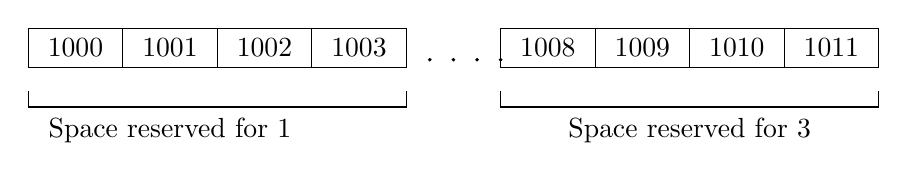
\begin{tikzpicture}
  \foreach \x in {0, ..., 3}
  \draw (\x*1.2cm, 0) -- +(1.2cm, 0) -- +(1.2cm, 0.5cm) -- +(0, .5cm) --
  cycle;
  \node at(5.1cm, .1cm) [circle,fill,inner sep=.5pt](a){};
  \node at(5.4cm, .1cm) [circle,fill,inner sep=.5pt](a){};
  \node at(5.7cm, .1cm) [circle,fill,inner sep=.5pt](a){};
  \node at(6cm, .1cm) [circle,fill,inner sep=.5pt](a){};
  \foreach \x in {0, ..., 3}
  \draw (\x*1.2cm+6cm, 0) -- +(1.2cm, 0) -- +(1.2cm, 0.5cm) -- +(0, .5cm) --
  cycle;
  \foreach \x [evaluate=\x as \xeval using \x+1000] in {0, ..., 3}
  \node at(\x*1.2cm + .6cm, .25cm) {\pgfmathtruncatemacro{\yet}{\xeval}\yet};
  \foreach \x [evaluate=\x as \xeval using \x+1008] in {0, ..., 3}
  \node at(\x*1.2cm+6.6cm, .25cm) {\pgfmathtruncatemacro{\yet}{\xeval}\yet};

  \draw (0, -.3cm) -- (0, -.5cm) -- (4.8cm, -.5cm) -- (4.8cm, -.3cm);
  \draw (6cm, -.3cm) -- (6cm, -.5cm) -- (10.8cm, -.5cm) -- (10.8cm, -.3cm);

  \node at (1.8cm, -.8cm) {Space reserved for 1};
  \node at (8.4cm, -.8cm) {Space reserved for 3};
\end{tikzpicture}
\caption{An Array's Memory Diagram}
\label{fig:An Array's Memory Diagram}
\end{center}
\end{figure}

Array elements are always(not always but most commonly. It is so common that I
have used always.) accessed using their indices so order of retrieval is $O(1)$
.(This is known as big-$O$ notation. You can find it in any Data Structure and
Algorithm book. The above program will not compile using old compilers which do
not support C99 standard like Turbo C++. Also, you may require to pass the flag
\texttt{-std=c99} or \texttt{-std=c11} to some versions of \texttt{gcc}. For
variable length arrays it is not necessary to declare the size in
advance. Even, input to program from other sources will do.

\begin{minted}[frame=single]{c}
#include <stdio.h>

int main()
{
  int i=0;

  printf("Enter the value of i:\n");
  scanf("%d", &i);
  getchar();
  char c[i];

  printf("Enter a string which contains one less no. of chars than i:\n");
  gets(c);
  puts(c);

  return 0;
}
\end{minted}
and the output is:
\\\\\texttt{Enter the value of i:\\
6\\
Enter a string which contains one less no. of chars than i:\\
shiv\\
shiv\\\\}
As you can see variable length array should be declared after the size is known
otherwise you may see strange output even though it is not compilation
error. For example you could have declaraed array immediately after \texttt{i}
but you will get some garbage output. The reason for this is that at that point
of time \texttt{i} contains garbage value. Also, note that array indices are
integers. Floating-point numbers or variables cannot be indices.

Now the question is why variable length arrays cannot initialized. If the size
of array is known at compile time then array can be initialized. The problem
with variable length array is that the variable's value may be in program or
come from user input. If it comes from user input then there is no way for
compiler to know that at compile time. Thus, to maintain consistency variable
length arrays are not initialized even if that variable has been assigned to in
the code.

Let us say you are writing a big piece of code and array is declared somewhere
and you want to know how many elemnets you can fill in the array or what is the
maximum size of array then you can use the following program:

\begin{minted}[frame=single]{c}

#include <stdio.h>

int main()
{
  float f[10]={0.0};

  printf("Size of array f is %zu.\n", sizeof(f)/sizeof(float));

  return 0;
}
\end{minted}
xand the output is:
\\\\\texttt{Size of array f is 10.\\\\}
Now an experienced programmer may ask that if we can know the size of array
then why we do not have something like out of bounds exception(i.e. accessing
elements having position beyong the size of array) of Java in C. My
answer to that is C was written in 1970 and Java in 1990. For example, there
are certain compilers with flags which help you detect this at runtime. You can
use \texttt{-fsanitize=address} which will help you detect the out of bounds
exception.

There are various ways in which you can define character arrays. For example,
\texttt{char c[6]={'h', 'e', 'l', 'l', 'o', '\textbackslash 0'};}. Remember, you must
terminate a character array with a null terminator. Another way to define the
same is: \texttt{char str[6] = "hello";}. In this example you do not need to
add \texttt{'\textbackslash 0'} explicitly as it is added automatically. Also, 6 is optional
here if you want you can ommit that. Of course second example is more
preferable. Note that if you declare an array of size \texttt{m} and data type
size of array is \texttt{n} bytes then the array will consume \texttt{m*n}
bytes no matter what; even when you are not using those bytes. Note that all
these arrays are on stack memory area. We will see how to allocate array(in
form of pointers) on heap memory area once we have studied pointers.

\section{Multi-Dimensional Arrays}
Arrays can be n-dmensional. There is no limit on dimensions. You can allocate
as much as your memory allows. We will begin with two-dimensional array. A
two-dimensional array looks like a matrix. Say a two-dimensional array has
\texttt{m} as one dimension and \texttt{n} as second diemnsion. Then total
no. of elements will be \texttt{m*n} and size occupied is \texttt{m*n*size of
  data type} of array. There are various ways to initialize a two-dimensional
array. Consider the following example:

\begin{minted}[frame=single]{c}
#include <stdio.h>

int main()
{
  int a[2][2] = {{1,2},{3,4}};
  int b[2][2] = {1,2,3,4};

  //iterating over array
  for(int i=0;i<2;i++)
  {
    for(int j=0;j<2;j++)
      printf("%d ", a[i][j]);
    printf("\n");
  }
  for(int i=0;i<2;i++)
  {
    for(int j=0;j<2;j++)
      printf("%d ", b[i][j]);
    printf("\n");
  }

  return 0;
}
\end{minted}
and the output is:
\\\\\texttt{1 2\\
3 4\\
1 2\\
3 4\\\\}
Thus, you see that allocation is first for latter dimension. Same holds trur
for more than 2 dimensions. Typical usage of two dimensional arrays is in
representation of structures which have a matrix representation, array of
strings, system of linear equations etc. For example, a csv file can be
represented by a two dimensional matrix.

Same way you can have multi-dimensional array. I leave it up to you to find
applications of different arrays. For now, try multiplying two matrices, doing
a transpose, inverse of a matrix and printing a yearly calenday for any year
for example. With the current information given to you, you should be able to
do all these easily. As shown for array a it is not really a single array but
an array of array. How we can read this is array a has two arrays each of which
have two integers.

\section{Pointers}
A pointer can store an address. A pointer of some type can store address of
that type and a pointer to void can store address of any type. Pointers are
possibly most powerful construct among all. Pointers are very much similar like
arrays in the sense that they also require contguous memory locations to be
available for allocation. Also, pointers can also be accessed like arrays using
subscript([ ]) operator.

There are four standard library functions associated with them. All these are
declared in \texttt{stdlib.h} which is part of standard c library. The
functions are: \texttt{malloc(), calloc(), realloc()} and
\texttt{free()}. Following is the contents of man pages verbatim,later in the
program you can go to opengroup links as well. Given below are signatures of
these functions:

\begin{minted}[frame=single]{c}
void *calloc(size_t nmemb, size_t size);
void *malloc(size_t size);
void free(void *ptr);
void *realloc(void *ptr, size_t size);
\end{minted}

here \texttt{size\_t} is the unsigned integer type of the result of the
\texttt{sizeof} operator. It is defined in \texttt{stddef.h}.
Descriptions from man page are given below:

\texttt{calloc()} allocates memory for an array of nmemb elements of
\texttt{size} bytes each and returns a pointer to the allocated memory. The
memory is set to zero. If \texttt{nmemb} or size is 0, then \texttt{calloc()}
returns either \texttt{NULL}, or a unique pointer value that can later be
successfully passed to \texttt{free()}.

\texttt{malloc()} allocates \texttt{size} bytes and returns a pointer to the
allocated memory. The memory is not cleared. If \texttt{size} is 0, then
\texttt{malloc()} returns either \texttt{NULL}, or a unique pointer value that
can later be successfully passed to \texttt{free()}.

\texttt{free()} frees the memory space pointed to by \texttt{ptr}, which must
have been returned by a previous call to \texttt{malloc(), calloc()} or
\texttt{realloc()}. Otherwise, or if \texttt{free(ptr)} has already been called
before, undefined behavior occurs. If \texttt{ptr} is \texttt{NULL}, no
operation is performed.

\texttt{realloc()} changes the size of the memory block pointed to by
\texttt{ptr} to \texttt{size} bytes. The contents will be unchanged to the
minimum of the old and new sizes; newly allocated memory will be
uninitialized. If \texttt{ptr} is \texttt{NULL}, then the call is equivalent to
\texttt{malloc(size)}, for all values of \texttt{size}; if \texttt{size} is
equal to zero, and \texttt{ptr} is not \texttt{NULL}, then the call is
equivalent to \texttt{free(ptr)}. Unless \texttt{ptr} is \texttt{NULL}, it must
have been returned by an earlier call to \texttt{malloc(), calloc()} or
\texttt{realloc()}. If the area pointed to was moved, a \texttt{free(ptr)} is
done.

Let us consider a program:

\begin{minted}[frame=single]{c}
#include <stdio.h>
#include <stdlib.h>

int main()
{
  int *p = NULL;

  p = (int*)malloc(sizeof(int)*8);

  for(int i=0;i<8;i++)
  {
    *(p+i)=i;
    printf("Content at %dth location is %d.\n", i, *(p+i));
  }

  return 0;
}
\end{minted}
and the output is:
\\\\\texttt{Content at 0th location is 0.\\
Content at 1th location is 1.\\
Content at 2th location is 2.\\
Content at 3th location is 3.\\
Content at 4th location is 4.\\
Content at 5th location is 5.\\
Content at 6th location is 6.\\
Content at 7th location is 7.\\\\}
We could have written the same program in a different way using subscript
operator as shown below:

\begin{minted}[frame=single]{c}
#include <stdio.h>
#include <stdlib.h>

int main()
{
  int *p = NULL;

  p = (int*)malloc(sizeof(int)*8);

  for(int i=0;i<8;i++)
  {
    p[i]=i;
    printf("Content at %dth location is %d.\n", i, p[i]);
  }

  return 0;
}
\end{minted}

A postfix expression followed by an expression in square brackets \texttt{[]}
is a subscripted designation of an element of an array object. The definition
of the subscript operator \texttt{[]} is that \texttt{E1[E2]} is identical to
\texttt{(*((E1)+(E2)))}. Because of the conversion rules that apply to the
binary \texttt{+} operator, if \texttt{E1} is an array object (equivalently, a
pointer to the initial element of an array object) and \texttt{E2} is an
integer, \texttt{E1[E2]} designates the \texttt{E2}-th element of \texttt{E1}
(counting from zero).

\subsection{Pointer Arithmetic}
Addition and subtarction of pointers was not covered in the chapter of
operators and 
expressions. When an expression that has integer type is added to or subtracted
from a pointer, the result has the type of the pointer operand. If the pointer
operand points to an element of an array object, and the array is large enough,
the result points to an element offset from the original element such that the
difference of the subscripts of the resulting and original array elements
equals the integer expression. In other words, if the expression \texttt{P}
points to the \texttt{i}-th element of an array object, the expressions
\texttt{(P)+N} (equivalently, \texttt{N+(P)}) and \texttt{(P)-N} (where
\texttt{N} has the value \texttt{n}) point to, respectively, the
\texttt{i+n}-th and \texttt{i-n}-th elements of the array object, provided they
exist. Moreover, if the expression \texttt{P} points to the last element of an
array object, the expression \texttt{(P)+1} points one past the last element of
the array object, and if the expression \texttt{Q} points one past the last
element of an array object, the expression \texttt{(Q)-1} points to the last
element of the array object. If both the pointer operand and the result point
to elements of the same array object, or one past the last element of the array
object, the evaluation will not produce an overflow; otherwise, the behavior is
undefined. If the result points one past the last element of the array object,
it will not be used as the operand of a unary \texttt{*} operator that is
evaluated.

When two pointers are subtracted, both shall point to elements of the same
array object, or one past the last element of the array object; the result is
the difference of the subscripts of the two array elements. The size of the
result is implementation-defined, and its type (a signed integer type) is
\texttt{ptrdiff\_t} defined in the \texttt{\textless stddef.h\textgreater}
header. If the result is not representable in an object of that type, the
behavior is undefined. In other words, if the expressions \texttt{P} and
\texttt{Q} point to, respectively, the \texttt{i}-th and \texttt{j}-th elements
of an array object, the expression \texttt{(P)-(Q)} has the value \texttt{i-j}
provided the value fits in an object of type \texttt{ptrdiff\_t}. Moreover, if
the expression \texttt{P} points either to an element of an array object or one
past the last element of an array object, and the expression \texttt{Q} points
to the last element of the same array object, the expression
\texttt{((Q)+1)-(P)} has the same value as \texttt{((Q)-(P))+1} and as
\texttt{-((P)-((Q)+1))}, and has the value zero if the expression \texttt{P}
points one past the last element of the array object, even though the
expression \texttt{(Q)+1} does not point to an element of the array object.

An example is given below:

\begin{minted}[frame=single]{c}
#include <stdio.h>
#include <stdlib.h>

int main()
{
  int *p = (int*)malloc(sizeof(int)*2);
  p[0] = 1;
  p[1] = 2;

  printf("%p %p\n", &p[0], &p[1]);
  printf("%td %td\n", &(p[0]) - &(p[1]), &(p[1]) - &p[0]);
  free(p);

  return 0;
}
\end{minted}
and the output is:
\\\\\texttt{0x7f8b5b404b10 0x7f8b5b404b14\\
-1 1\\\\}
As you can see the absolute values of addresses differ by 4 but when converted
to difference it is divided by size of data type or is given by differebce in
position.

You can also apply increment and decrement operators on pointers. I will show
you a reimplementation of previos program using increment operator:

\begin{minted}[frame=single]{c}
#include <stdio.h>
#include <stdlib.h>

int main()
{
  int *p = NULL;

  p = (int*)malloc(sizeof(int)*8);
  int *q = p;

  for(int i=0;i<8;i++)
  {
    *(p+i)=i;
    printf("Content at %dth location is %d.\n", i, *(q++));
  }

  return 0;
}
\end{minted}
and the output is:
\\\\\texttt{Content at 0th location is 0.\\
Content at 1th location is 1.\\
Content at 2th location is 2.\\
Content at 3th location is 3.\\
Content at 4th location is 4.\\
Content at 5th location is 5.\\
Content at 6th location is 6.\\
Content at 7th location is 7.\\\\}

\section{Address-of and Indirection Operators}
As is the case with subscript operator and pointer arithmetic in the fourth
chapter that I have delayed these two as well for I wanted to put them
here. Whenever you declare a plain variable you have an address associated with
it and that variable is an lvalue. Just to repeat an lvalue is a value whose
address can be taken. To take the address of an lvalue you use the address
operator which is \texttt{\&}. Now a pointer points to address of any value as
we know so we can use address operator to get the address and use a pointer to
store. There are several usage of storing an address. Most notable of those is
pass-by-address which we will see in next chapter which will deal with
functions. Let us say we take address of a variable and assign that to a
pointer. Then if we change the value of the memory pointed to by the pointer
then the variable whose address has been taken will get updated with this new
value. Consider for example:

\begin{minted}[frame=single]{c}
#include <stdio.h>

int main()
{
  int  i = 8;
  int *p = &i;

  *p = 7;

  printf("i=%d *p=%d\n", i, *p);

  return 0;
}
\end{minted}
and the output is:
\\\\\texttt{i=7 *p=7\\\\}
Note that since both \texttt{i} and \texttt{p} are sharing address as
\texttt{p} is assigned the address of \texttt{i} changing the value of one will
have effect on the other. For exmaple:

\begin{minted}[frame=single]{c}
#include <stdio.h>

int main()
{
  int  i = 8;
  int *p = &i;

  *p = 7;

  printf("i=%d *p=%d\n", i, *p);

  *p = 10;

  printf("i=%d *p=%d\n", i, *p);

  return 0;
}
\end{minted}
and the output is:
\\\\\texttt{i=7 *p=7\\
i=10 *p=10\\\\}
So you see the power of pointers that if you have an address you can modify its
contents. This is exacly what \texttt{scanf()} does. The dereference operator
or indirection operator or asterisk (\texttt{*}) gives you value at address
pointed to by pointer o. However, if you want to change address of some varible
like that ofi by doing something like \texttt{\&i=\&someOthervar;} you cannot do that
because address is not an lvalue. However, you can pass address of a pointer
variable to some other function and use it using pointer to pointer notation
which I will show you in next chapter. As I have shown pointers are kind of
equivalent to array except the fact that they are on heap and sizeof operator
will not work on them. Consider this example:

\begin{minted}[frame=single]{c}
#include <stdio.h>
#include <stdlib.h>

int main()
{
  int  a[4] = {1,2,3,4};
  int* p    = a;
  int* q    = (int*)calloc(10, 4);

  for(int i=0; i<4; i++)
    printf("i=%d *p=%d\n", i, *(p+i));

  printf("Size of a=%d\n", sizeof(a));
  printf("Size of p=%d\n", sizeof(p));
  printf("Size of q=%d\n", sizeof(q));

  return 0;
}
\end{minted}
and the output is:
\\\\\texttt{i=0 *p=1\\
i=1 *p=2\\
i=2 *p=3\\
i=3 *p=4\\
Size of a=16\\
Size of p=4\\
Size of q=4\\\\}
Here \texttt{p} acts as pointer to array. You can have a pointer to any kind of
array. You can point to any element of array because array elements are lvalues
whose addresses can be taken and to initialize a pointer alll you need is an
address.

Complex pointer arithmetic is best avoided. Be very thoughtful that if you
really really need it. Use loops to iterate arrays. Multiple levels of
indirection is also bad. Typically I have not seen more than pointers to
pointers. Now we will see array of pointers.

\section{Arrays of Pointers}
Pointers are like ordinary variables in many ways, so we can as well create
array of pointers. Consider following for example:

\begin{minted}[frame=single]{c}
#include <stdio.h>
#include <stdlib.h>

int main()
{
  char* strArray[2]={"Hello", "Universe!"};

  for(int i=0; i<2; i++)
    printf("%s\n", strArray[i]);

  return 0;
}
\end{minted}
and the output is:
\\\\\texttt{Hello\\
Universe!\\\\}
Note how the length of two array elements are different as they are
pointers. Let us do a more complex example:

\begin{minted}[frame=single]{c}
#include <stdio.h>
#include <stdlib.h>

int main()
{
  int* intArray[2];

  intArray[0] = (int*)calloc(3, sizeof(int));
  intArray[1] = (int*)calloc(2, sizeof(int));

  *intArray[0]     = 4;
  *(intArray[0]+1) = 5;
  *(intArray[0]+2) = 6;


  *intArray[1]     = 1;
  *(intArray[1]+1) = 2;

  for(int i=0; i<3; i++)
  {
    printf("Memory location=%p Content=%d\n", intArray[0]+i, *(intArray[0]+i));
  }

  for(int i=0; i<2; i++)
  {
    printf("Memory location=%p Content=%d\n", intArray[1]+i, *(intArray[1]+i));
  }

  return 0;
}
\end{minted}
and the output is:
\\\\\texttt{Memory location=0x87d1008 Content=4\\
Memory location=0x87d100c Content=5\\
Memory location=0x87d1010 Content=6\\
Memory location=0x87d1018 Content=1\\
Memory location=0x87d101c Content=2\\\\\\}
Note missing four bytes between 6 and 1. Memory locations may be different on
your system. But see how messy pointer syntax can go even with such simple
code. Array to pointers are useful for containing variables of dynamic size of
same type.

\section{Pointers of Pointers}
Pointers to pointers are same as array of pointers. The only difference is that
you can dynamically modify the number of elements. Consider the following
example:

\begin{minted}[frame=single]{c}
#include <stdio.h>
#include <stdlib.h>

int main()
{
  int** intPtr;

  intPtr = (int**)malloc(sizeof(sizeof(int*)*2));

  *intPtr = (int*)malloc(sizeof(int)*3);
  *(intPtr+1) = (int*)malloc(sizeof(int)*4);

  **intPtr     = 1;
  *(*intPtr+1) = 2;
  *(*intPtr+2) = 7;


  **(intPtr+1)      = 3;
  *(*(intPtr+1)+1)  = 5;
  *(*(intPtr+1)+2)  = 9;
  *(*(intPtr+1)+3)  = 11;

  for(int i=0; i<3; i++)
    printf("Memory location=%p content=%d\n", *intPtr+i, *(*intPtr+i));

  for(int i=0; i<4; i++)
    printf("Memory location=%p content=%d\n", *(intPtr+1)+i, *(*(intPtr+1)+i));

  return 0;
}
\end{minted}
and the output is:
\\\\\texttt{Memory location=0x9947018 content=1\\
Memory location=0x994701c content=2\\
Memory location=0x9947020 content=7\\
Memory location=0x9947028 content=3\\
Memory location=0x994702c content=5\\
Memory location=0x9947030 content=9\\
Memory location=0x9947034 content=11\\\\}
Again memory location may change on your system. As you can see how things can
get messy with pointers. Believe me you will hate this. Also, I do not see any
reason to use more than two levels of indirection. So you get the idea. If you
need dynamic no. of elements with dynamic content you are going to use pointers
to pointers.

\section{\texttt{realloc()} Function}
Once \texttt{malloc()} and \texttt{calloc()} allocate some memory you have that
certain amount of memory available to you. When you have an array you have some
memory but what if you want more later. \texttt{reallloc()} comes to rescue
you. Here is a sample program:

\begin{minted}[frame=single]{c}
#include <stdio.h>
#include <stdlib.h>

int main()
{
  int *p = (int*)malloc(sizeof(int)*2);

  *p     = 5;
  *(p+1) = 7;

  printf("Original 1st element=%d\n", *p);
  printf("Original 2nd element=%d\n", *(p+1));

  p = (int*)realloc(p, sizeof(int)*4);

  *(p+2) = 9;
  *(p+3) = 11;

  printf("New 1st element=%d\n", *p);
  printf("New 2nd element=%d\n", *(p+1));
  printf("New 3rd element=%d\n", *(p+2));
  printf("New 4th element=%d\n", *(p+3));

  return 0;
}
\end{minted}
and the output is:
\\\\\texttt{Original 1st element=5\\
Original 2nd element=7\\
New 1st element=5\\
New 2nd element=7\\
New 3rd element=9\\
New 4th element=11\\\\}

\section{\texttt{free} Function}
Whatever program we have written in this chapter related to dynamic memory
allocation using malloc() etc are bad code just because we are not releasing
memory properly. Any call to memory allocation functions have to be matched
with a corresponding free() call. The reason for this is that when all pointers
to a memory area are lost and that memory is not freed then operating system
cannot recycle that memory. In case of servers or long running processes this
may eat up all the physical RAM and virtual memory and eventually freeze the
system. To guard against such events you must macth all allocation calls with
deallocation calls so that operating system can reclaim the freed memmory.

You must heed this warning given here with all of your focus. You got to handle
heap that is dynamically allocated memory yourself. You allocate and you free
it. If you miss you have a memory leak.

\section{Constness of Pointers}
To make anything constant you need to associate const keyword with it. For
example, \texttt{const int i; const float f;}. However, with pointers in
picture scenarios change compared to two simple previous examples. When
pointers are made constant there are two elements. First is the pointer itself
and second is the value pointed to. Consider for example:

\begin{minted}[frame=single]{c}
const int* i;  //constant pointer data is not
int* const i;  //constant data pointer is not
const int* const i; //both are const
\end{minted}
The way to read it is you draw a vertical line where asterisk(\texttt{*}) is
there and the value associated with const is constant. Whenever you need use a
constant freely. Try to use constants more and more. Also, prefre them to
following:

\begin{minted}[frame=single]{c}
#define MAX 10
\end{minted}

It will replace \texttt{MAX} with 10 in the file everywhere without any concern
of type-safety. Also, it does not enter in the symbol table so while debugging
you will not see \texttt{MAX} anywhere. So instead you should use something
like:

\begin{minted}[frame=single]{c}
const int MAX=10;
\end{minted}

I will also like to say something about volatile variables. Beginners are
usually convinced that volatile variables cannot be declraed as const. Let me
iterate the definitions once again. A const variable cannot be modifed by the
program itself. A volatile variable can be modified by sources other than the
program itself. Hence, a const volatile variable cannot be modified by the
program but other sources can still modify it.

\chapter{Functions}
I know that you will readily agree with me if I say that humans get bored if
they have to do same things again and again. I know you get bored too and I too
get bored. We all. We as humans have this built-in nature that repititive
things are just not fit for us. Also, as a human being our capacity to
understand large things at once is difficult. We understand small-small things
and build large chunk based on those small things. Dennis Ritchie perhaps had
known this. I am saying because C has got something called functions. C
functions allow you to split a big logic into small ones and therefore
facilitating modular programming. They also form the basis of strutctured
programming the very base which made C popular. There is also something called
recursion which is a very poewrful tool. In this chapter we will also see how
to do multifile programming. I cannot emphasize much that how important it is
that you master the technique of functions well and not to mention function
pointers which can do the magic. I will show you the very glimpse only. I can
show you the way but walking on that is your job. It is upto you to do the
actual work. I have kept things simple and minimal with a pupose. I do not want
you to get bogged down with a thick and heavy book. All my examples are toy
examples but you have seen things can get somehwat complex.

We have already seen the special \texttt{main()} function.

Given below are typical code for a function:

\begin{Verbatim}[frame=single]
//function prototype
return-type function-name(argument list); //here varible names may be ommitted

//function body
return-type function-name(argument list) //variable names cannot be ommitted``
{
  //your code here

  //call some other function
  function-name(arugment-list-without-type);

  return value-of-return-type;
}
\end{Verbatim}
This might be a bit abstract but please bear it a bit.

\section{Pass by Value}

Consider a program which adds two numbers and let us say that you may need to
add lots of them.

\begin{minted}[frame=single]{c}
#include <stdio.h>

void add(int first_integer, int second_integer)
{
  printf("%d+%d=%d\n", first_integer, second_integer, first_integer + second_integer);
}

int main()
{
  int a=5, b=7;

  add(a, b);

  return 0;
}
\end{minted}
Note that you need function body before its use else you need at least a
function prototype before use. If you do not do so you will get a compiler
warnign. An example is given below:

\begin{minted}[frame=single]{c}
#include <stdio.h>

//not how argument names are not required
void add(int, int);

int main()
{
  int a=5, b=7;

  add(a, b);

  return 0;
}

void add(int first_integer, int second_integer)
{
  printf("%d+%d=%d\n", first_integer, second_integer, first_integer + second_integer);
}
\end{minted}
output is same as above.

When a function is called a stack frame is created for that function. The
control is passed to that function. When a return statement is encountered or
end of that function is reached, the function returns. The local variables of
the caller function are saved on stack and thus their value is restored from
that value unless the address of those variables are passed.

What you have seen just above is known as pass-by-value. In this case a copy of
parameters is made and passed on to called function by caller function. So, if
called function makes a change to values then those are not reflected back in
the caller function. As an example I will use famous example of swapping values
of two variables. First, I will show how pass-by-value works. So here is the
code:

\begin{minted}[frame=single]{c}
#include <stdio.h>

void swap(int, int);

int main()
{
  int a=5, b=7;

  printf("Before swap a=%d and b=%d\n", a, b);
  swap(a, b);
  printf("After swap a=%d and b=%d\n", a, b);

  return 0;
}

void swap(int first_integer, int second_integer)
{
  int temp=first_integer;
  first_integer=second_integer;
  second_integer=temp;
}
\end{minted}
and the output is:
\\\\\texttt{Before swap a=5 and b=7\\
After swap a=5 and b=7}

\section{Pass by Address}
\label{section:Pass by address}
The output of previous program was not exactly what we wanted. The solution is
to pass-by-address. When you the address to a called function, it receives
address in a pointer variable. Then if it modifies the value stored at that
address then it is reflected back in the caller. Let us see an example to
understand:

\begin{minted}[frame=single]{c}
#include <stdio.h>

void swap(int*, int*);

int main()
{
  int a=5, b=7;

  printf("Before swap a=%d and b=%d\n", a, b);
  swap(&a, &b);
  printf("After swap a=%d and b=%d\n", a, b);

  return 0;
}

void swap(int* first_int, int* second_int)
{
  int temp=*first_int;
  *first_int=*second_int;
  *second_int=temp;
}
\end{minted}
and the output is:
\\\\\texttt{Before swap a=5 and b=7\\
After swap a=7 and b=5\\\\}
When you pass address of a variable the change is maintained at that address
and thus when the control is returned the values are changed.

\section{Passing Arrays}
Arrays are always passed by address because if they are passed by value then
they will eat upprevious real-estate of little stack memory. Now since they
are passed by address by default base address of the array is passed. This
also implied that changes made to the array by the called function will be
reflected in caller after the call is complete. Passing arrays around various
functions is easy but requires extra piece of information to be sent to the
called function from column because the when an array is passed it is always
passed as a pointer or in other words the array becomes a pointer. Thus you
need to pass the length of array if you want the
called function to iterate or traverse over the array. Given below is a simple
example demonstrating this:

\begin{minted}[frame=single]{c}
#include <stdio.h>

void f(int *a, int n)
{
  for(size_t i=0; i<n; ++i)
    printf("%d\n", a[i]);
}

int main()
{
  int a[10]={0, 1, 2, 3, 4, 5, 6, 7, 8, 9};
 
  f(a, 10);
  
  return 0;
}
\end{minted}

and the output is easy to guess. The program prints 0 through 9, each on a
separate line.

However, this is not the only way to send an array to function. The other
solution could be to send start and end element as pointer. Since we are
already sending first element as pointer if we have end element's address we
can iterate over the array with ease. This is demonstrated in the next
program:

\begin{minted}[frame=single]{c}
#include <stdio.h>

void f(int *a, int *end )
{
  for(int *p=a; p!=end; ++p)
    printf("%d\n", *p);
  printf("%d\n", *end);
}

int main()
{
  int a[10]={0, 1, 2, 3, 4, 5, 6, 7, 8, 9};
 
  f(a, &a[9]);
  
  return 0;
}
\end{minted}
Note that we need to print last element separately because loop will not
execute its code for the last element. This is cumbersome but does equivalent
work as the previous program.

However, passing two dimensional array is different. If you want to pass an
array of the form \texttt{a[m][n]} then it would be passed as \texttt{int
  (*)[n]}. Thus passing is not that you will pass \texttt{int **}. Following
code shows how to pass and print a two dimensional array:

\begin{minted}[frame=single]{c}
void f(int a[][2], unsigned int fd, unsigned int sd)
{
  for(unsigned int i=0; i<fd; ++i)
  {
    for(unsigned int j=0; j<sd; ++j)
    {
      printf("%d ", a[i][j]);
    }
    printf("\n");
  }
}

int main()
{
  int a[5][2]={{0, 1}, {2, 3}, {4, 5}, {6, 7}, {8, 9}};
 
  f(a, 5, 2);
  
  return 0;
}
\end{minted}
and the output is:
\\\\\texttt{0 1\\
2 3\\
4 5\\
6 7\\
8 9\\
\\\\}
Note that array type changes to \texttt{int (*)[2]}, similarly an array of form
\texttt{a[l][m][n]} will change its type to \texttt{int (*)[m][n]}.

We have already seen pass by address but what if we want to pass to pointers
and change the pointer itself. In the example shown in the
\autoref{section:Pass by address} \nameref{section:Pass by address} we have two
variables on stack whose addresses were passed and the values were swapped
which was contained on those addresses. Can we extrapolate this to change
addresses themselves. Let us see an example:

\begin{minted}[frame=single]{c}
#include <stdio.h>

void f(int *p, int *q)
{
  int *temp = p;

  p = q;
  q = temp;
}

int main()
{
  int i=5, j=10;
  int *p=&i, *q=&j;

  f(p, q);

  printf("%d %d\n", *p, *q);
  return 0;
}
\end{minted}
and the output is:
\\\\\texttt{5 10\\\\}
Now as we say the pointers are still pointing to original values. The reason is
because when we call function \texttt{f} and pass addresses of \texttt{i} and
\texttt{j} then a copy of those addresses are sent. If we want to swap the
values by swapping pointers then we have to send addresses of pointers. The
program is shown below:

\begin{minted}[frame=single]{c}
#include <stdio.h>

void f(int **p, int **q)
{
  int *temp = *p;

  *p = *q;
  *q = temp;
}

int main()
{
  int i=5, j=10;
  int *p=&i, *q=&j;

  f(&p, &q);

  printf("%d %d\n", *p, *q);
  return 0;
}
\end{minted}

Now since the pointers themselves are swapped it is easy to guess the output
and it is \texttt{10 5}. Notice since we are sending addresses of pointers we
have to receive them using pointer to pointer syntax.

\section{Recursion}
In C recusion is the concept of a function calling itself. When a repeated
operation has to be preformed over a variable, recursion can be used. Recursion
simplifies the code a lot. Typically there is always a more effective iterative
solutions are available but there are certain cases where recursion is always
better than iteration. For example, traversal of trees where iteration is not
so effective as compared to recursion. For beginners it is hard to understand
recursion but once you understand it then it is not that hard to
understand. The first example I am going to give is that of factorials. The
formula for factorial is given by $n!=\prod_{k=1}^{n}i$  and recursive
definition of factorial is given by:

$$\begin{array}{rl}n!=\left\{\begin{array}{ll}1&\hspace{1em}\text{if
    n=0}\\[4pt](n-1)!\ast n&\hspace{1em}\text{if
    n>0}\end{array}\right.\end{array}$$

Note that every recursion has to be written carefully in thse sense that it
must have a termination condition and that in all the cases the termination
condition must be reached. If a recursion is too deep or infinite there will be
a stack overlow and the program will terminate. First, I will show you an
iterative version with a function. Let us try to compute factorial of an
integer:

\begin{minted}[frame=single]{c}
#include <stdio.h>

long long fact(int input);

int main()
{
  int input=0;

  printf("Enter a number whose input has to be computed:\n");
  scanf("%d", &input);

  printf("Factorial of %d is %lld.\n", input, fact(input));

  return 0;
}

long long fact(int input)
{
  long long output=1;
  while(input!=0)
  {
    output*=input;
    input--;
  }

  return output;
}
\end{minted}
and the output is:
\\\\\texttt{Enter a number whose factorial has to be computed:\\
17\\
Factorial of 17 is 355687428096000.\\\\}
Now we will see the recursive version:

\begin{minted}[frame=single]{c}
#include <stdio.h>

long long fact(int input);

int main()
{
  int input=0;

  printf("Enter a number whose factorial has to be computed:\n");
  scanf("%d", &input);

  printf("Factorial of %d is %lld.\n", input, fact(input));

  return 0;
}

long long fact(int input)
{
  if(input==0)
    return 1;
  else
    return fact(input-1)*input;
}
\end{minted}
and the output is:
\\\\\texttt{Enter a number whose factorial has to be computed:\\
16\\
Factorial of 16 is 20922789888000.\\\\}
Recursion is very simple yet may be very deceptive to understand for
beginners. Let us dissect the code. Our input was 16 so \texttt{input} will not
match and \texttt{return fact(15)*16;} will be executed. Here, before
\texttt{fact(16)} can return \texttt{fact(15)} has to return. And, similarly
before \texttt{fact(15)} can return \texttt{fact(14)} has to return. Now, note
that for \texttt{fact(0)} there is no such condition and it can return 1 making
it possible for \texttt{fact(1)} to return, which, in turn will make it posible
for \texttt{fact(2)} to return and so on. So, what is happening is function is
calling itself by creating more and more function frames and when the
termination condition reaches the stack unwinds.

Let us consider one more famous example for recursive function, that is of
computing Fibonacci numbers. The Fibonacci series is given by:

$$F_n = F_{n-1} + F_{n-2}$$

where first two numebrs are given by:

$$ F_0 = 0 \text{~and~} F_1 = 1$$ or
$$ F_0 = 1 \text{~and~} F_1 = 1$$

First, consider the iterative version:

%\chapter{GNU Free Documentation License}
\phantomsection  % so hyperref creates bookmarks
%\label{label_fdl}

 \begin{center}

       Version 1.3, 3 November 2008


 Copyright \copyright{} 2000, 2001, 2002, 2007, 2008  Free Software Foundation, Inc.
 
 \bigskip
 
     \texttt{<http://fsf.org/>}
  
 \bigskip
 
 Everyone is permitted to copy and distribute verbatim copies
 of this license document, but changing it is not allowed.
\end{center}


\begin{center}
{\bf\large Preamble}
\end{center}

The purpose of this License is to make a manual, textbook, or other
functional and useful document ``free'' in the sense of freedom: to
assure everyone the effective freedom to copy and redistribute it,
with or without modifying it, either commercially or noncommercially.
Secondarily, this License preserves for the author and publisher a way
to get credit for their work, while not being considered responsible
for modifications made by others.

This License is a kind of ``copyleft'', which means that derivative
works of the document must themselves be free in the same sense.  It
complements the GNU General Public License, which is a copyleft
license designed for free software.

We have designed this License in order to use it for manuals for free
software, because free software needs free documentation: a free
program should come with manuals providing the same freedoms that the
software does.  But this License is not limited to software manuals;
it can be used for any textual work, regardless of subject matter or
whether it is published as a printed book.  We recommend this License
principally for works whose purpose is instruction or reference.


\begin{center}
{\Large\bf 1. APPLICABILITY AND DEFINITIONS\par}
\phantomsection
\addcontentsline{toc}{section}{1. APPLICABILITY AND DEFINITIONS}
\end{center}

This License applies to any manual or other work, in any medium, that
contains a notice placed by the copyright holder saying it can be
distributed under the terms of this License.  Such a notice grants a
world-wide, royalty-free license, unlimited in duration, to use that
work under the conditions stated herein.  The ``\textbf{Document}'', below,
refers to any such manual or work.  Any member of the public is a
licensee, and is addressed as ``\textbf{you}''.  You accept the license if you
copy, modify or distribute the work in a way requiring permission
under copyright law.

A ``\textbf{Modified Version}'' of the Document means any work containing the
Document or a portion of it, either copied verbatim, or with
modifications and/or translated into another language.

A ``\textbf{Secondary Section}'' is a named appendix or a front-matter section of
the Document that deals exclusively with the relationship of the
publishers or authors of the Document to the Document's overall subject
(or to related matters) and contains nothing that could fall directly
within that overall subject.  (Thus, if the Document is in part a
textbook of mathematics, a Secondary Section may not explain any
mathematics.)  The relationship could be a matter of historical
connection with the subject or with related matters, or of legal,
commercial, philosophical, ethical or political position regarding
them.

The ``\textbf{Invariant Sections}'' are certain Secondary Sections whose titles
are designated, as being those of Invariant Sections, in the notice
that says that the Document is released under this License.  If a
section does not fit the above definition of Secondary then it is not
allowed to be designated as Invariant.  The Document may contain zero
Invariant Sections.  If the Document does not identify any Invariant
Sections then there are none.

The ``\textbf{Cover Texts}'' are certain short passages of text that are listed,
as Front-Cover Texts or Back-Cover Texts, in the notice that says that
the Document is released under this License.  A Front-Cover Text may
be at most 5 words, and a Back-Cover Text may be at most 25 words.

A ``\textbf{Transparent}'' copy of the Document means a machine-readable copy,
represented in a format whose specification is available to the
general public, that is suitable for revising the document
straightforwardly with generic text editors or (for images composed of
pixels) generic paint programs or (for drawings) some widely available
drawing editor, and that is suitable for input to text formatters or
for automatic translation to a variety of formats suitable for input
to text formatters.  A copy made in an otherwise Transparent file
format whose markup, or absence of markup, has been arranged to thwart
or discourage subsequent modification by readers is not Transparent.
An image format is not Transparent if used for any substantial amount
of text.  A copy that is not ``Transparent'' is called ``\textbf{Opaque}''.

Examples of suitable formats for Transparent copies include plain
ASCII without markup, Texinfo input format, LaTeX input format, SGML
or XML using a publicly available DTD, and standard-conforming simple
HTML, PostScript or PDF designed for human modification.  Examples of
transparent image formats include PNG, XCF and JPG.  Opaque formats
include proprietary formats that can be read and edited only by
proprietary word processors, SGML or XML for which the DTD and/or
processing tools are not generally available, and the
machine-generated HTML, PostScript or PDF produced by some word
processors for output purposes only.

The ``\textbf{Title Page}'' means, for a printed book, the title page itself,
plus such following pages as are needed to hold, legibly, the material
this License requires to appear in the title page.  For works in
formats which do not have any title page as such, ``Title Page'' means
the text near the most prominent appearance of the work's title,
preceding the beginning of the body of the text.

The ``\textbf{publisher}'' means any person or entity that distributes
copies of the Document to the public.

A section ``\textbf{Entitled XYZ}'' means a named subunit of the Document whose
title either is precisely XYZ or contains XYZ in parentheses following
text that translates XYZ in another language.  (Here XYZ stands for a
specific section name mentioned below, such as ``\textbf{Acknowledgements}'',
``\textbf{Dedications}'', ``\textbf{Endorsements}'', or ``\textbf{History}''.)  
To ``\textbf{Preserve the Title}''
of such a section when you modify the Document means that it remains a
section ``Entitled XYZ'' according to this definition.

The Document may include Warranty Disclaimers next to the notice which
states that this License applies to the Document.  These Warranty
Disclaimers are considered to be included by reference in this
License, but only as regards disclaiming warranties: any other
implication that these Warranty Disclaimers may have is void and has
no effect on the meaning of this License.


\begin{center}
{\Large\bf 2. VERBATIM COPYING\par}
\phantomsection
\addcontentsline{toc}{section}{2. VERBATIM COPYING}
\end{center}

You may copy and distribute the Document in any medium, either
commercially or noncommercially, provided that this License, the
copyright notices, and the license notice saying this License applies
to the Document are reproduced in all copies, and that you add no other
conditions whatsoever to those of this License.  You may not use
technical measures to obstruct or control the reading or further
copying of the copies you make or distribute.  However, you may accept
compensation in exchange for copies.  If you distribute a large enough
number of copies you must also follow the conditions in section~3.

You may also lend copies, under the same conditions stated above, and
you may publicly display copies.


\begin{center}
{\Large\bf 3. COPYING IN QUANTITY\par}
\phantomsection
\addcontentsline{toc}{section}{3. COPYING IN QUANTITY}
\end{center}


If you publish printed copies (or copies in media that commonly have
printed covers) of the Document, numbering more than 100, and the
Document's license notice requires Cover Texts, you must enclose the
copies in covers that carry, clearly and legibly, all these Cover
Texts: Front-Cover Texts on the front cover, and Back-Cover Texts on
the back cover.  Both covers must also clearly and legibly identify
you as the publisher of these copies.  The front cover must present
the full title with all words of the title equally prominent and
visible.  You may add other material on the covers in addition.
Copying with changes limited to the covers, as long as they preserve
the title of the Document and satisfy these conditions, can be treated
as verbatim copying in other respects.

If the required texts for either cover are too voluminous to fit
legibly, you should put the first ones listed (as many as fit
reasonably) on the actual cover, and continue the rest onto adjacent
pages.

If you publish or distribute Opaque copies of the Document numbering
more than 100, you must either include a machine-readable Transparent
copy along with each Opaque copy, or state in or with each Opaque copy
a computer-network location from which the general network-using
public has access to download using public-standard network protocols
a complete Transparent copy of the Document, free of added material.
If you use the latter option, you must take reasonably prudent steps,
when you begin distribution of Opaque copies in quantity, to ensure
that this Transparent copy will remain thus accessible at the stated
location until at least one year after the last time you distribute an
Opaque copy (directly or through your agents or retailers) of that
edition to the public.

It is requested, but not required, that you contact the authors of the
Document well before redistributing any large number of copies, to give
them a chance to provide you with an updated version of the Document.


\begin{center}
{\Large\bf 4. MODIFICATIONS\par}
\phantomsection
\addcontentsline{toc}{section}{4. MODIFICATIONS}
\end{center}

You may copy and distribute a Modified Version of the Document under
the conditions of sections 2 and 3 above, provided that you release
the Modified Version under precisely this License, with the Modified
Version filling the role of the Document, thus licensing distribution
and modification of the Modified Version to whoever possesses a copy
of it.  In addition, you must do these things in the Modified Version:

\begin{itemize}
\item[A.] 
   Use in the Title Page (and on the covers, if any) a title distinct
   from that of the Document, and from those of previous versions
   (which should, if there were any, be listed in the History section
   of the Document).  You may use the same title as a previous version
   if the original publisher of that version gives permission.
   
\item[B.]
   List on the Title Page, as authors, one or more persons or entities
   responsible for authorship of the modifications in the Modified
   Version, together with at least five of the principal authors of the
   Document (all of its principal authors, if it has fewer than five),
   unless they release you from this requirement.
   
\item[C.]
   State on the Title page the name of the publisher of the
   Modified Version, as the publisher.
   
\item[D.]
   Preserve all the copyright notices of the Document.
   
\item[E.]
   Add an appropriate copyright notice for your modifications
   adjacent to the other copyright notices.
   
\item[F.]
   Include, immediately after the copyright notices, a license notice
   giving the public permission to use the Modified Version under the
   terms of this License, in the form shown in the Addendum below.
   
\item[G.]
   Preserve in that license notice the full lists of Invariant Sections
   and required Cover Texts given in the Document's license notice.
   
\item[H.]
   Include an unaltered copy of this License.
   
\item[I.]
   Preserve the section Entitled ``History'', Preserve its Title, and add
   to it an item stating at least the title, year, new authors, and
   publisher of the Modified Version as given on the Title Page.  If
   there is no section Entitled ``History'' in the Document, create one
   stating the title, year, authors, and publisher of the Document as
   given on its Title Page, then add an item describing the Modified
   Version as stated in the previous sentence.
   
\item[J.]
   Preserve the network location, if any, given in the Document for
   public access to a Transparent copy of the Document, and likewise
   the network locations given in the Document for previous versions
   it was based on.  These may be placed in the ``History'' section.
   You may omit a network location for a work that was published at
   least four years before the Document itself, or if the original
   publisher of the version it refers to gives permission.
   
\item[K.]
   For any section Entitled ``Acknowledgements'' or ``Dedications'',
   Preserve the Title of the section, and preserve in the section all
   the substance and tone of each of the contributor acknowledgements
   and/or dedications given therein.
   
\item[L.]
   Preserve all the Invariant Sections of the Document,
   unaltered in their text and in their titles.  Section numbers
   or the equivalent are not considered part of the section titles.
   
\item[M.]
   Delete any section Entitled ``Endorsements''.  Such a section
   may not be included in the Modified Version.
   
\item[N.]
   Do not retitle any existing section to be Entitled ``Endorsements''
   or to conflict in title with any Invariant Section.
   
\item[O.]
   Preserve any Warranty Disclaimers.
\end{itemize}

If the Modified Version includes new front-matter sections or
appendices that qualify as Secondary Sections and contain no material
copied from the Document, you may at your option designate some or all
of these sections as invariant.  To do this, add their titles to the
list of Invariant Sections in the Modified Version's license notice.
These titles must be distinct from any other section titles.

You may add a section Entitled ``Endorsements'', provided it contains
nothing but endorsements of your Modified Version by various
parties---for example, statements of peer review or that the text has
been approved by an organization as the authoritative definition of a
standard.

You may add a passage of up to five words as a Front-Cover Text, and a
passage of up to 25 words as a Back-Cover Text, to the end of the list
of Cover Texts in the Modified Version.  Only one passage of
Front-Cover Text and one of Back-Cover Text may be added by (or
through arrangements made by) any one entity.  If the Document already
includes a cover text for the same cover, previously added by you or
by arrangement made by the same entity you are acting on behalf of,
you may not add another; but you may replace the old one, on explicit
permission from the previous publisher that added the old one.

The author(s) and publisher(s) of the Document do not by this License
give permission to use their names for publicity for or to assert or
imply endorsement of any Modified Version.


\begin{center}
{\Large\bf 5. COMBINING DOCUMENTS\par}
\phantomsection
\addcontentsline{toc}{section}{5. COMBINING DOCUMENTS}
\end{center}


You may combine the Document with other documents released under this
License, under the terms defined in section~4 above for modified
versions, provided that you include in the combination all of the
Invariant Sections of all of the original documents, unmodified, and
list them all as Invariant Sections of your combined work in its
license notice, and that you preserve all their Warranty Disclaimers.

The combined work need only contain one copy of this License, and
multiple identical Invariant Sections may be replaced with a single
copy.  If there are multiple Invariant Sections with the same name but
different contents, make the title of each such section unique by
adding at the end of it, in parentheses, the name of the original
author or publisher of that section if known, or else a unique number.
Make the same adjustment to the section titles in the list of
Invariant Sections in the license notice of the combined work.

In the combination, you must combine any sections Entitled ``History''
in the various original documents, forming one section Entitled
``History''; likewise combine any sections Entitled ``Acknowledgements'',
and any sections Entitled ``Dedications''.  You must delete all sections
Entitled ``Endorsements''.

\begin{center}
{\Large\bf 6. COLLECTIONS OF DOCUMENTS\par}
\phantomsection
\addcontentsline{toc}{section}{6. COLLECTIONS OF DOCUMENTS}
\end{center}

You may make a collection consisting of the Document and other documents
released under this License, and replace the individual copies of this
License in the various documents with a single copy that is included in
the collection, provided that you follow the rules of this License for
verbatim copying of each of the documents in all other respects.

You may extract a single document from such a collection, and distribute
it individually under this License, provided you insert a copy of this
License into the extracted document, and follow this License in all
other respects regarding verbatim copying of that document.


\begin{center}
{\Large\bf 7. AGGREGATION WITH INDEPENDENT WORKS\par}
\phantomsection
\addcontentsline{toc}{section}{7. AGGREGATION WITH INDEPENDENT WORKS}
\end{center}


A compilation of the Document or its derivatives with other separate
and independent documents or works, in or on a volume of a storage or
distribution medium, is called an ``aggregate'' if the copyright
resulting from the compilation is not used to limit the legal rights
of the compilation's users beyond what the individual works permit.
When the Document is included in an aggregate, this License does not
apply to the other works in the aggregate which are not themselves
derivative works of the Document.

If the Cover Text requirement of section~3 is applicable to these
copies of the Document, then if the Document is less than one half of
the entire aggregate, the Document's Cover Texts may be placed on
covers that bracket the Document within the aggregate, or the
electronic equivalent of covers if the Document is in electronic form.
Otherwise they must appear on printed covers that bracket the whole
aggregate.


\begin{center}
{\Large\bf 8. TRANSLATION\par}
\phantomsection
\addcontentsline{toc}{section}{8. TRANSLATION}
\end{center}


Translation is considered a kind of modification, so you may
distribute translations of the Document under the terms of section~4.
Replacing Invariant Sections with translations requires special
permission from their copyright holders, but you may include
translations of some or all Invariant Sections in addition to the
original versions of these Invariant Sections.  You may include a
translation of this License, and all the license notices in the
Document, and any Warranty Disclaimers, provided that you also include
the original English version of this License and the original versions
of those notices and disclaimers.  In case of a disagreement between
the translation and the original version of this License or a notice
or disclaimer, the original version will prevail.

If a section in the Document is Entitled ``Acknowledgements'',
``Dedications'', or ``History'', the requirement (section~4) to Preserve
its Title (section~1) will typically require changing the actual
title.


\begin{center}
{\Large\bf 9. TERMINATION\par}
\phantomsection
\addcontentsline{toc}{section}{9. TERMINATION}
\end{center}


You may not copy, modify, sublicense, or distribute the Document
except as expressly provided under this License.  Any attempt
otherwise to copy, modify, sublicense, or distribute it is void, and
will automatically terminate your rights under this License.

However, if you cease all violation of this License, then your license
from a particular copyright holder is reinstated (a) provisionally,
unless and until the copyright holder explicitly and finally
terminates your license, and (b) permanently, if the copyright holder
fails to notify you of the violation by some reasonable means prior to
60 days after the cessation.

Moreover, your license from a particular copyright holder is
reinstated permanently if the copyright holder notifies you of the
violation by some reasonable means, this is the first time you have
received notice of violation of this License (for any work) from that
copyright holder, and you cure the violation prior to 30 days after
your receipt of the notice.

Termination of your rights under this section does not terminate the
licenses of parties who have received copies or rights from you under
this License.  If your rights have been terminated and not permanently
reinstated, receipt of a copy of some or all of the same material does
not give you any rights to use it.


\begin{center}
{\Large\bf 10. FUTURE REVISIONS OF THIS LICENSE\par}
\phantomsection
\addcontentsline{toc}{section}{10. FUTURE REVISIONS OF THIS LICENSE}
\end{center}


The Free Software Foundation may publish new, revised versions
of the GNU Free Documentation License from time to time.  Such new
versions will be similar in spirit to the present version, but may
differ in detail to address new problems or concerns.  See
\texttt{http://www.gnu.org/copyleft/}.

Each version of the License is given a distinguishing version number.
If the Document specifies that a particular numbered version of this
License ``or any later version'' applies to it, you have the option of
following the terms and conditions either of that specified version or
of any later version that has been published (not as a draft) by the
Free Software Foundation.  If the Document does not specify a version
number of this License, you may choose any version ever published (not
as a draft) by the Free Software Foundation.  If the Document
specifies that a proxy can decide which future versions of this
License can be used, that proxy's public statement of acceptance of a
version permanently authorizes you to choose that version for the
Document.


\begin{center}
{\Large\bf 11. RELICENSING\par}
\phantomsection
\addcontentsline{toc}{section}{11. RELICENSING}
\end{center}


``Massive Multiauthor Collaboration Site'' (or ``MMC Site'') means any
World Wide Web server that publishes copyrightable works and also
provides prominent facilities for anybody to edit those works.  A
public wiki that anybody can edit is an example of such a server.  A
``Massive Multiauthor Collaboration'' (or ``MMC'') contained in the
site means any set of copyrightable works thus published on the MMC
site.

``CC-BY-SA'' means the Creative Commons Attribution-Share Alike 3.0
license published by Creative Commons Corporation, a not-for-profit
corporation with a principal place of business in San Francisco,
California, as well as future copyleft versions of that license
published by that same organization.

``Incorporate'' means to publish or republish a Document, in whole or
in part, as part of another Document.

An MMC is ``eligible for relicensing'' if it is licensed under this
License, and if all works that were first published under this License
somewhere other than this MMC, and subsequently incorporated in whole
or in part into the MMC, (1) had no cover texts or invariant sections,
and (2) were thus incorporated prior to November 1, 2008.

The operator of an MMC Site may republish an MMC contained in the site
under CC-BY-SA on the same site at any time before August 1, 2009,
provided the MMC is eligible for relicensing.


\begin{center}
{\Large\bf ADDENDUM: How to use this License for your documents\par}
\phantomsection
\addcontentsline{toc}{section}{ADDENDUM: How to use this License for your documents}
\end{center}

To use this License in a document you have written, include a copy of
the License in the document and put the following copyright and
license notices just after the title page:

\bigskip
\begin{quote}
    Copyright \copyright{}  YEAR  YOUR NAME.
    Permission is granted to copy, distribute and/or modify this document
    under the terms of the GNU Free Documentation License, Version 1.3
    or any later version published by the Free Software Foundation;
    with no Invariant Sections, no Front-Cover Texts, and no Back-Cover Texts.
    A copy of the license is included in the section entitled ``GNU
    Free Documentation License''.
\end{quote}
\bigskip
    
If you have Invariant Sections, Front-Cover Texts and Back-Cover Texts,
replace the ``with \dots\ Texts.''\ line with this:

\bigskip
\begin{quote}
    with the Invariant Sections being LIST THEIR TITLES, with the
    Front-Cover Texts being LIST, and with the Back-Cover Texts being LIST.
\end{quote}
\bigskip
    
If you have Invariant Sections without Cover Texts, or some other
combination of the three, merge those two alternatives to suit the
situation.

If your document contains nontrivial examples of program code, we
recommend releasing these examples in parallel under your choice of
free software license, such as the GNU General Public License,
to permit their use in free software.

\backmatter
\printindex
\end{document}
